%Slovak version of QGIS documantation - DRAFT
%modificated qgis_user_guide.tex
%translated by Lubos Balazovic (balazovic at mailbox dot sk)
%used encoding: iso-8859-2

\documentclass[10pt,slovak]{timthesis}

\usepackage{geometry}
\geometry{verbose,letterpaper,tmargin=1in,bmargin=1in,lmargin=1in,rmargin=
1in}
\usepackage{helvet}
\usepackage[T1]{fontenc}
\usepackage[latin1]{inputenc}
\usepackage{setspace}
\usepackage{paralist}
\usepackage{color}
\usepackage{hyperref}
 \hypersetup{backref,colorlinks=true}
\usepackage{ae,aecompl}
\usepackage{graphicx}
\usepackage{picins}
\usepackage{fancyhdr}
\usepackage{extramarks}
\usepackage{makeidx}
\usepackage{datetime}
\pagestyle{empty}
%define tip float
\usepackage{float}
\floatstyle{ruled}
\newfloat{Tip}{H}{lox}
\floatname{Tip}{Tip}
\newcommand\qgistip[1]{\raggedright\small{#1}}
\renewcommand{\topfraction}{0.85}
 \renewcommand{\textfraction}{0.1}
\renewcommand{\floatpagefraction}{0.75}




\makeindex
%Added by Tim to define a month year date style
\newdateformat{mydate}{\monthname[\THEMONTH] \THEYEAR}
%\renewcommand\familydefault{lucidabrightsans}
\title{
\includegraphics[scale=0.4]{qgis_user_guide_images/qgis_icon_new_verylarge}\\
Pou�vate�sk� pr�ru�ka Quantum GIS\\
\large Verzia 0.7 \textsl{'Seamus'}}
\author{Gary E. Sherman \\Tim Sutton \\Radim Bla�ek (GRASS) \\ Lars Luthman (GPS modul)\\
\date{\mydate\today}
}


\begin{document}
\pagenumbering{roman}

% To disable first line indents of paragraphs after the first one
\setlength{\parindent}{0in}


\maketitle
\tableofcontents
\listof{Tip}{Zoznam QGIS tipov}
\newpage
%\newpage
%added by Tim to create a decent space between paragraphs
%note its only after toc so toc remains compact
\setlength{\parskip}{8pt plus 1pt minus 1pt}
%\fancyfoot[C]{\thepage}
\pagestyle{fancy}
\fancyhead[L]{Pou��vate�sk� pr�ru�ka QGIS}
\fancyhead[R]{\textsl{Verza 0.7}}

\pagenumbering{arabic}
\begin{onehalfspace}
\reversemarginpar
\input{forward_sk.tex}
%
\chapter{Introduction}

Welcome to the wonderful world of Geographical Information Systems (GIS)!
Quantum GIS (QGIS) is an Open Source Geographic Information System. The project
was born in May of 2002 and was established as a project on SourceForge in June
of the same year. We've worked hard to make GIS software (which is traditionaly
expensive commerical software) a viable prospect for anyone with basic access
to a Personal Computer. QGIS currently runs on most Unix platforms, Window, and
OS X. QGIS is developed using the Qt toolkit (\url{http://www.trolltech.com})
and C++. This means that QGIS feels snappy to use and has a pleasing, easy to
use graphical user interface. 

QGIS aims to be an easy to use GIS, providing common functions and features.
The initial goal was to provide a GIS data viewer. QGIS has reached that point
in its evolution and is being used by many for their daily GIS data viewing
needs. QGIS supports a number of raster and vector data formats, with new
support easily added using the plugin architecture (see Appendix
\ref{appdx_data_formats} for a full list of currenly supported data formats).
QGIS is released under the GNU Public License (GPL). Devloping QGIS under this
license means that you can (if you want to) inspect and modify the source code
and guarantees that you, our happy user will always have access to a GIS
program that is free of cost and can be freely modified. You should have
received a full copy of the license with your copy of QGIS, and is also
available as Appendix \ref{gpl_appendix}.  
\begin{quote}
\begin{center}
\textbf{Note:} The latest version of this document can always be found at \newline
http://qgis.sourceforge.net/docs/userguide.html 
\end{center}
\end{quote}

\section{Major Features}

QGIS has many common GIS features and functions. The major features
are listed below. 

\begin{compactenum}
\item Support for spatially enabled PostgreSQL tables using PostGIS 
\item Support for ESRI shapefiles and other vector formats support by the
OGR library, including MapInfo files 
\item GRASS integration, including view, edit, and analysis
\item On the fly projection of vector layers
\item Map composer
\item Identify features 
\item Display attribute table 
\item Select features 
\item Label features
\item Persistent selections 
\item Save and restore projects
\item Support for raster formats supported by the GDAL library 
\item Change vector symbology (single, graduated, unique value, and continuous) 
\item SVG markers symbology (single, unique value, and graduated) 
\item Display raster data such as digital elevation models, aerial photography
or landsat imagery 
\item Change raster symbology (grayscale, pseudocolor and multiband RGB) 
\item Export to Mapserver map file 
\item Digitizing support
\item Map overview
\item Plugins 
\end{compactenum}


\section{Whats New in 0.7}
Version 0.7 brings several important features, including projection support, a map composer, and better integration with GRASS. The major new features in this release include:
\begin{compactenum}
  \item On the fly projection for reprojecting layers in different coordinate systems
  \item Map Composer for creating print layouts
  \item Toolbox for running GRASS tools from QGIS
  \item Raster graphing tool to produce a histogram for a raster layer.
  \item Raster query using the identify tool to get the pixel
  values from a raster 
  \item New customizable settings for the digitizing line width, color, and selection color  
  \item New symbols for use with point layers are available from the layer properties dialog 
  \item Spatial bookmarks allow you to create and manage bookmarks for an area on the map
  \item Measure tool to measure distances on the map with both
  segment length and total length displayed as you click
  \item GPX loading times and memory consumption for large GPX (GPS) files
  has been drastically reduced.  
  \item Digitizing enhancements, including the ability to capture data straight
  into PostgreSQL/PostGIS, and improvements to the definition of attribute tables
  for newly created layers.
  \item Raster Georeferencing plugin can be used
  to generate a world file for a raster by defining known
  control points in the raster coordinate system.
\end{compactenum}

 not translated yet
%documentation for 0.6 (not updated for 0.7 yet)
%translated by Lubos Balazovic (balazovic at mailbox dot sk)
%used encoding: iso-8859-2
% TODO list
% * Capture localized screenshots 
% * Update for 0.7

\chapter{Prv� kroky}

T�to kapitola V�m pod� r�chly preh�ad ako funguje QGIS a ako mo�no vysk��a� vzorku �dajov dostupn� z webovej str�nky QGIS-u.


\section{In�tal�cia}
\index{In�tal�cia}
In�tal�cia QGIS-u je op�san� v pr�lohe \ref{install_guide}. In�tala�n� pr�ru�ka sa ��ri spolu so zdrojov�m k�dom QGIS-u a taktie� je dostupn� na str�nke \url{http://qgis.org}. Pre platformy Windows a Mac OSX existuje QGIS v podobe �tandardn�ho in�tal��n�ho in�tala�n�ho bal�ka.


\section{Vzorky �dajov} \index{�daje!vzorky} Pokia� nem�te po ruke �iadne GIS 
�daje, m��ete si stiahnu� vzorku obsahuj�cu �dajov� s�pravu Alja�ka z webovej 
str�nky QGIS-u na \url{http://qgis.org}. �dajov� s�prava Alja�ka bude sl��i� ako z�klad pre mnoh� pr�klady a sn�mky obrazovky uv�dzan� v tomto dokumente.


\section{Spustenie QGIS}

V pr�pade, �e je QGIS nain�talovan� v adres�ri, ku ktor�mu je v premennej PATH nastaven� cesta, sta�� na jeho spustenie nap�sa� do pr�kazov�ho riadku: \textbf{qgis} alebo pou�i� dvojklik na odkaz na ploche smeruj�ci ku aplik�cii QGIS. Pod MS Windows, spust�te QGIS pou�it�m menu �tart a pr�slu�n�ho odkazu; pod Mac OSX, dvojklikom na ikonu v prie�inku va�ich aplik�ci�.

%\begin{figure}
%\caption{QGIS Main Window}
%\end{figure} 
\subsection{Parametre pr�kazov�ho riadku}\index{parametre pr�kazov�ho riadku}
QGIS sp��tan� z pr�kazov�ho riadku podporuje mno�stvo parametrov. Zoznam t�chto parametrov  je mo�n� z�ska� s pou�it�m pr�kazu \texttt{qgis ---help}. Preh�ad ich pou�itia v QGIS-e vyzer� taktoormul�ci:
\small
\begin{verbatim}
Pou�itie: /home/gsherman/qgis06_rc/bin/qgis [parametre] [S�BORY]
  parametre:
        [--snapshot s�bor]           vysiela sn�mky nahrat�ch �dajov�ch s�prav dan�ho s�boru
        [--lang jazyk]               pou�it� jazykov� mut�cia
        [--project projektov�_s�bor] nahr� dan� QGIS projekt
        [--help]                     zobraz� tento text (v angli�tine -- pozn. prekl.)
  S�BORY:
    S�bory �pecifikovan� v pr�kazovom riadku m��u by� s�bormi rastrov�mi,
    vektorov�mi, a s�bormi projektov QGIS (.qgs):
     1. Rastrov� s�bory - podporovan� form�ty s� GeoTiff, DEM
        a ostatn� podporovan� kni�nicou GDAL
     2. Vektorov� s�bory - podpororvan� form�ty s� ESRI Shape s�bory
        a ostatn� podporovan� kni�nicou OGR a PostgreSQL vrstvy s pou�it�m 
        roz��renia PostGIS 

\end{verbatim}
\normalsize
\begin{Tip} \caption{\textsc{Pr�klad na pou�itie parametrov pr�kazov�ho riadku}}
\qgistip{
Qgis je mo�n� spusti� aj tak, �e do pr�kazov�ho riadku zad�me jeden, alebo viac �dajov�ch s�borov. Napr�klad, na to, aby sa okam�ite nahrali dva shape s�bory a jeden rastrov� s�bor, v pr�pade pokia� QGIS sp���ame z adres�ra, kde sa na�e s�bory s �dajmi nach�dzaj�, pou�ijeme pr�kaz: 
\ttfamily{	qgis ak\_shade.tif alaska.shp majrivers.shp}
}
\end{Tip}

\section{Hlavn� okno QGIS-u}\index{hlavn� okno}

Akon�hle sa QGIS spust�, prich�dzate do kontaktu s jeho hlavn�m okno v podobe ako je zobrazen� pod t�mto textom.

\begin{figure}[h]
   \begin{center}
   \caption{Hlavn� okno}\label{fig:startup}
   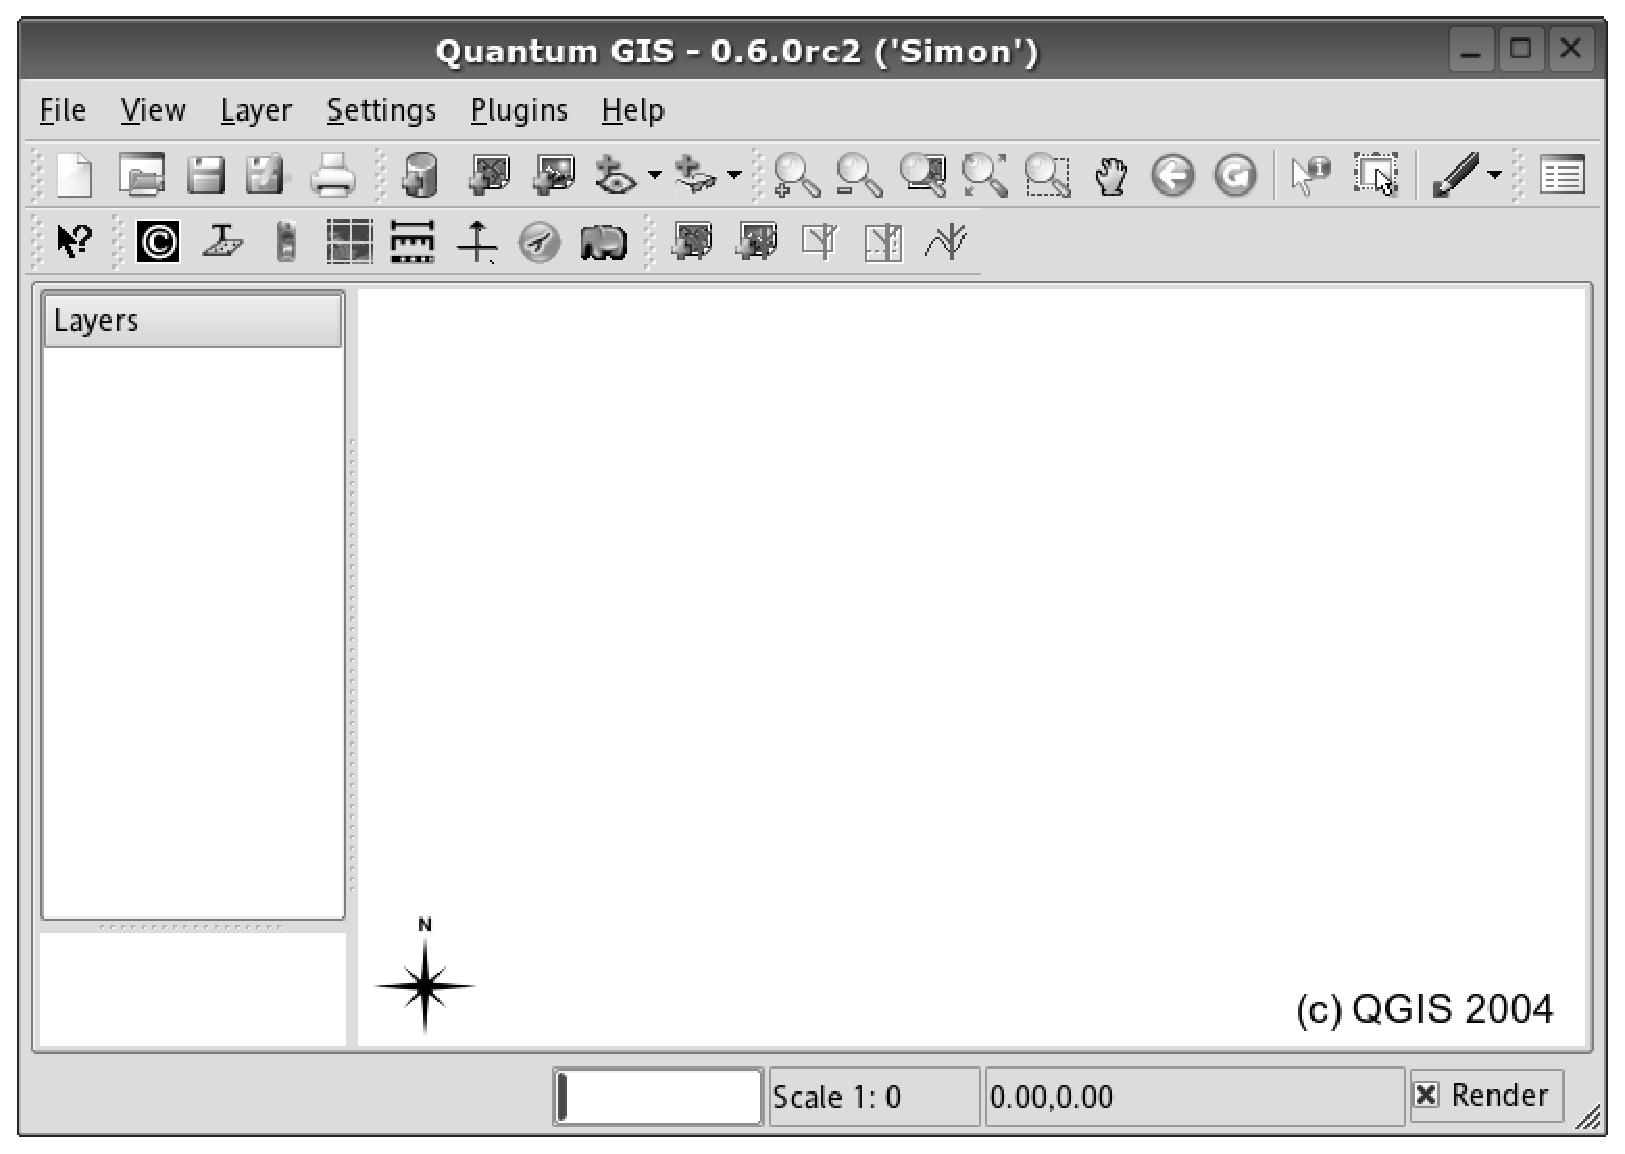
\includegraphics[scale=.5]{qgis_user_guide_images/startup}
\end{center}  
   
\end{figure}
\textsc{Pozn�mka -- vzh�ad dekor�cie okien (tituln� li�ta at�.) sa m��u na va�om po��ta�i l��i�, z�visia toti� od opera�n�ho syst�mu a spr�vcu okien}
Hlavn� okno QGIS-u je rozdelen� do �iestich oblast�:

\begin{compactenum}
\item Hlavn� menu
\item N�strojov� li�ta
\item Mapov� legenda
\item Mapov� pl�tno
\item Panel Preh�ad
\item Stavov� riadok
\end{compactenum}

T�mto �iestim komponentom rozhrania QGIS-u sa bli��ie venuj� �al�ie �asti tohoto dokumentu.

\subsection{Hlavn� menu}
\index{menu}
Hlavn� menu poskytuje prostedn�ctvom �tandardn�ch okien hierarchick�ho menu pr�stup k r�znym funcki�m QGIS-u. Tu je zoznam menu na najvy��ej �rovni a zhrnutie niektor�ch funkci�, ktor� sprostredkuj�:
\begin{compactitem}
\item S�bor (otvorenie projektu, ulo�enie, export obr�zku, vlastnosti)
\item Vrstva (pridanie, zobrazenie a skrytie vrstvy)
\item Poh�ad (zoom, obnovenie poh�adu)
\item N�stroje (spr�vca z�suvn�ch modulov, vlastnosti)
\item Z�suvn� moduly (menu pridan� z�suvn�mi modulmi, ktor� s� nahrat�)
\item Pomocn�k (dokument�cia a web odkazy)
\end{compactitem}
%See Appendix \ref{app_menu} for complete descriptions of the menu items.

\subsection{N�strojov� li�ty}
\index{n�strojov� li�ty}
N�strojov� li�ty umo��uj� pr�stup k t�m najpou��vanej��m funkci�m z menu a mnoh�m �al��m n�strojom pre interakt�vnu pr�cu s mapou. Ku ka�dej polo�ke n�strojovej li�ty existuje rozba�ovacie pomocn� informa�n� text. Sta�� chv��u podr�a� my� nad nejakou polo�kou a �ochv��a sa objav� kr�tky popis n�stroja a jeho ��el. %See Appendix \ref{app_toolbar} for complete
%descriptions and illustrations of the various toolbars.  

\subsection{QGIS Mapov� legenda}
\index{legenda}
Oblas� mapovej legendy sa pou��va na nastavenie vidite�nosti a z-poradia vrstiev.
Z-poradie znamen�, �e v zozname vy��ie umiestnen� vrstvy legendy s� vykres�ovan� cez ni��ie vrstvy v zozname v legende. Za�krt�vacie pol��ko pri ka�dej polo�ke legendy sl��i na zobrazenie alebo skrytie tej-ktorej vrstvy.\index{vrstva!vidite�nos�}
\begin{Tip} \caption{\textsc{Zobrazenie menu vrstvy}}\index{vrstva!kontextov� menu}
\qgistip{Kontextov� menu pre �ubovo�n� vrstvu v legende m��ete zobrazi� v kliknut�m prav�m tla�idlom na meno vrstvy. Kontextov� menu pozost�va z polo�iek na pr�cu s vrstvou a vlastnost� jej zobrazenia.}
\end{Tip}

Pri ka�dej polo�ke legendy sa m��u objavi� nasleduj�ce mini ikony:

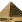
\includegraphics[scale=1]{qgis_user_guide_images/pyramid} Toto je rastrov� vrstva, ktor� m� na zv��enie efekt�vnosti vykres�ovania postaven� pyram�dy (pozri Sekciu \ref{raster_pyramids}).\\

\includegraphics[scale=1]{qgis_user_guide_images/no_pyramid} Toto je rastov� vrstva ktor� nem� �iadne pyram�dy (pozri Sekciu \ref{raster_pyramids}).\\

\includegraphics[scale=1]{qgis_user_guide_images/inoverview} T�to vrstva je zobrazovan� okrem hlavn�ho mapov�ho pl�tna aj v paneli Preh�ad.\\

\includegraphics[scale=1]{qgis_user_guide_images/editable} Toto je vektorov� vrstva, ktor� je moment�lne nastaven� ako upravovate�n�.\\
\subsection{QGIS Mapov� poh�ad}
\index{mapa!poh�ad}
Toto je 'pracovn� �as�' QGIS-u -- v tejto oblasti s� zobrazovan� mapy! Mapa zobrazen� v tomto okne z�vis� na vektorov�ch a rastrov�ch vrstv�ch, ktor� s� nahrat� (viac inform�ci� o tomto je v �al��ch �astiach dokumentu). Mapov� poh�ad sa d� pos�va� (je mo�n� zmeni� poh�ad posunut�m mapov�ho poh�adu na in� oblas� z�ujmu), pribli�ova� a vzdia�ova� (zoom) a podporuje r�zne �al�ie akcie tak ako s� uvednen� vo vy��ie op�san� v opise n�strojovej li�ty vy��ie.  Mapov� poh�ad a legenda s� navz�jom �zko previazan� -- mapy v poh�ade reaguj� na zmeny, vykonan� v legende...
\begin{Tip}\caption{\textsc{Zmena poh�adu kolieskom my�i}}\index{zoom!koliesko my�i}
\qgistip{S kolieskom my�i sa d� mapa pribli�ova� alebo vzda�ova�. Umiestnite kurzor my�i do oblasti mapy a ot��an�m kolieska dopredu (smerom od v�s) poh�ad pribli�ujete a opa�n�m smerom (smerom k v�m) vzda�ujete.
}
\end{Tip}
\subsection{QGIS panel Preh�ad}
\index{map!overview}
Oblas� mapov�ho preh�adu poskytuje celkov� poh�ad na vrstvy, ktor� boli do neho pridan�. �erven�m obd�nikom je vymedzen� rozsah (poloha) aktu�lneho mapov�ho poh�adu. To V�m umo��uje r�chlo zisti�, ktor� oblas� si pr�ve prezer�te. Majte na pam�ti, �e popisy v mapovom preh�ade nie s� zobrazovan� dokonca ani v pr�pade, ak je zapnut� zobrazovanie popisov v nastaven� vrstvy.

\subsection{QGIS stavov� riadok mapy} 
Stavov� riadok zobrazuje v mapov�ch s�radniciach (t.j. meteroch alebo desiatkov�ch stup�och) aktu�lnu polohu kurzora my�i v mapovom poh�ade. Stavov� riadok tie� tie� ukazuje rozsah mapov�ho poh�adu tak, ako ste ho posunuli, pribl��ili, �i vzdialili. Ukazovate� priebehu v stavovom riadku zobrazuje priebeh vykres�ovania ka�dej vrsty vykres�ovanej do mapov�ho poh�adu. V niektor�ch pr�padoch (ako je napr�klad zozbieranie �tatistiky v rastrov�ch vrstv�ch) sl��i ukazovate� priebehu na zobrazovanie priebehu �asovo n�ro�nej��ch oper�ci�. Na konci stavov�ho riadku je mal� za�krt�vacie pol��ko ktor� sa pou��va na do�asn� pozastavenie vykres�ovania vrstiev do mapov�ho poh�adu) pozri �alej -- �as� \ref{subsec:redraw_events}.

\section{Vykres�ovanie}\label{subsec:redraw_events}\index{rendering}
�tandardne QGIS vykres�uje v�etky vidite�n� vrstvy v�dy ke� je potrebn� obnovi� (aktualizova�) obraz mapov�ho pl�tna. Udalosti, ktor�ch d�sledkom je obnovenie mapov�ho pl�tna:
\begin{compactitem}
\item pridanie vrstvy
\item posun, alebo zmena ve�kos�i poh�adu 
\item zmena ve�kosti okna QGIS
\item zmena vidite�nosti vrstvy, alebo vrstiev
\end{compactitem}
QGIS v�m dovo�uje riadi� proces vykres�ovania viacer�mi sp�sobmi.

\subsection{Vykres�ovanie v z�vislosti od mierky}\index{rendering!vykres�ovanie v z�vislosti od mierky}
Vykres�ovanie v z�vislosti od mierky v�m umo��uje ur�i� minim�lnu a maxim�lnu mierku, v ktorej bude vrstva vidite�n�.  Nastavenie vykres�ovania v z�vislosti od mierky, n�jdete v menu vlastnosti, ktor� otvor�te dvojklikom na dan� vrstvu v legende. Na karte 
\textit{V�eobecn�} , nastavte hodnoty minim�lnej a maxim�lnej mierky a kliknite na za�rt�vacie pol��ko \textit{Pou�i� vykres�ovanie v z�vislosti od mierky}.

Hodnoty mierok je mo�n� zisti� pribl��en�m poh�adu na dan� ve�kos� a od��tan�m mierky zo stavov�ho riadku QGIS-u.
\index{mierka}
\subsection{Oval�danie mapov�ho vykres�ovania}
Mapov� vykres�ovanie sa d� ovl�da� nasleduj�cimi sp�sobmi:
\begin{compactenum}
\item Preru�enie vykres�ovania po�as vykres�ovania mapov�ho pl�tna
\item Do�asn� pozastavenie vykres�ovania
\item Nastavenie vo�by na ovl�danie vidite�nosti vrstiev prid�van�ch do mapy
\end{compactenum}
\subsection{Zastavenie vykres�ovania}\index{rendering!halting}
Vykres�ovania mapy je mo�n� zastavi� stla�en�m kl�vesy ESC. T�m sa zastav� obnovenie mapov�ho pl�tna a ostane mapa zostane len �iasto�ne vykreslen�. Medzi stla�en�m kl�vesy ESC a momentom, ke� bude vykres�ovanie mapy zastven� m��e ubehn�� ist� �as.
\subsection{Pozastavenie Vykres�ovania}\index{rendering!suspending}
Na pozastavenie vykres�ovania, kliknite na za�krt�vacie pol��ko \textit{Vykres�ovanie} v spodnom pravom horu stavov�ho riadku. Pokia� pol��ko \textit{Vykres�ovanie} nie za�krtnut�, QGIS mapov� pl�tno neprekre�uje v pr�pade �iadnej z udalost� op�san�ch v �asti
\ref{sec:redraw_events}. Pr�kladmi sit�ci�, ke� je u�ito�n� preru�i� vykres�ovanie s� napr.:
\begin{compactitem}
\item pridanie mnoh�ch vrstiev a nastavenie symboliky pre ne ich pred vykreslen�m
\item pridanie jednej alebo viac rozsiahlych vrstiev a nastavenie vykres�ovania v z�vislosti od mierky pred ich vykreslen�m
\item pridanie jednej alebo viac vrstiev a nastavenie osobitn�ho poh�adu pred ich vykreslen�m
\item �ubovo�n� kombin�cia vy��ie spoment�ch
\end{compactitem}
Za�krtnutie pol��ka \textit{Vykres�ovanie} zapne vykres�ovanie a pri�in� sa o okam�it� obnovenie mapov�ho pl�tna.
\subsection{Nastavenie vo�by prid�vania vrstvy}\index{vykres�ovanie!nastavenie}\index{vrstvy!po�iato�n� vidite�nos�}
Je mo�n� nastavi� vo�bu v�dy nahara� nov� vrstvy bez ich vykreslenia. To znamen�, �e vrstva bude pridan� do mapy, ale za�krt�vacie pol��ko jej vidite�nosti v legende bude nastaven� ako neza�krtnut�. T�to vo�ba sa d� nastavi� kliknit�m na kartu \textit{Vykres�ovanie} v menu \textit{Vlastnosti}, ktor� sa nach�dza v hlavnom menu pod polo�kou \textit{Nastavenia}. Tu za�krtnite pol��ko
\textit{Nov� vrstvy pridan� do mapy nie s� zobrazovan�}. Ka�d� vrstva prid�van� do mapy bude prednastaven� ako vypnut� (nevidite�n�).
\subsection{Aktualiz�cia zobrazenia mapy po�as vykres�ovania}\index{rendering!update
during drawing}
M��ete nastavi� vo�bu na aktualiz�ciu zobrazenia mapy v priebehu generovania objektov. �tandardne QGIS nerzobraz� �iadne objekty vrstvy, pokia� nie je vygenerovan� cel� vrstva. Aktualiz�ciu zobrazenia po�as na��tavania objektov zo zdroja �dajov sa d� nastavi� kliknut�m na kartu \textit{Vykres�ovanie}v menu \textit{Vlastnosti} nach�dzaj�com sa v polo�ke \textit{Nastavenia} z hlavn�ho menu. Tu sa nastav� po�et objektov na vhodn� hodnotu pre aktualiz�ciu zobrazenia po�as generovnia vrstvy. Nastavenie na 0 znemo�n� aktualiz�ciu po�as generovania (toto je predvolen� hodnota). Nastavenie pr�li� n�zkej hodnoty bude ma� za n�sledok n�zky v�kon, ke�e mapov� pl�tno bude priebe�ne aktualizovan� po�as na��tavania objektov. Odpor��a sa za�a� s hodnotou 500.

%% vim:autoindent:set textwidth=78:
\chapter{Working with Vector Data}
QGIS supports vector data in a number of formats, including shapefiles,
MapInfo mif, and PostGIS\index{PostGIS} layers in a PostgreSQL database. Support for
additional data types is provided by plugins, for example delimited
text\index{delimited text}.

This section describes how to work with two common formats:
shapefiles\index{shapefile} and PostGIS\index{PostGIS} layers. Many of the
features available in QGIS work the same regardless of the vector data source.
This is by design and includes the identify, select, labeling, and attributes
functions.

\section{Shapefiles}\index{shapefile}
Shapefile support is provided by a library of functions (OGR
\url{http://www.remotesensing.org/gdal/ogr})\index{ogr}. See Appendix
\ref{appdx_ogr} for a list of supported formats.

A shapefile actually consists of a minimum of three
files:\index{shapefile!format}
\begin{compactenum}
\item .shp file containing the feature geometries
\item .dbf file containing the attributes in dBase format
\item .shx index file
\end{compactenum}
The technical specification for the shapefile format can be found at\\
\url{http://www.esri.com/library/whitepapers/pdfs/shapefile.pdf}\index{shapefile!specification}.
\subsection{Loading a Shapefile}
\parpic[l]{
\includegraphics{qgis_user_guide_images/addshapefile}}To load a
shapefile, start QGIS and click on the \textit{Add a vector layer} toolbar bar
button\index{shapefile!loading}. This same tool can be used to load any of the
formats supported by the OGR library.

Clicking on the tool brings up a standard open file dialog (Figure
\ref{fig:openshapefile}) which allows you to navigate the file system and load
a shapefile (or other supported data source).  You can also select the
Encoding type for the shapefile if desired.
\begin{figure}[h]
   \begin{center}
   \caption{Open OGR Data Source Dialog}\label{fig:openshapefile}\smallskip
   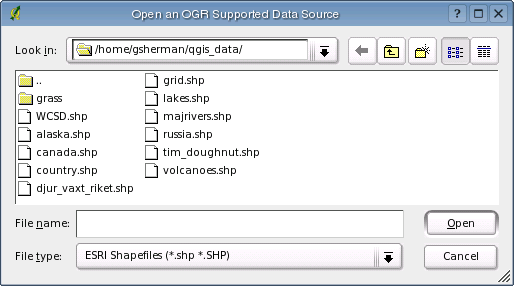
\includegraphics[scale=.75]{qgis_user_guide_images/shapefileopendialog}
\end{center}  
   
\end{figure}
Selecting a shapefile from the list and clicking Ok loads it into QGIS. Figure
\ref{fig:loadedshapefile} shows QGIS after loading the country.shp file.
\begin{figure}[h]
   \begin{center}
   \caption{QGIS with the countries Shapefile Loaded}\label{fig:loadedshapefile}\smallskip
   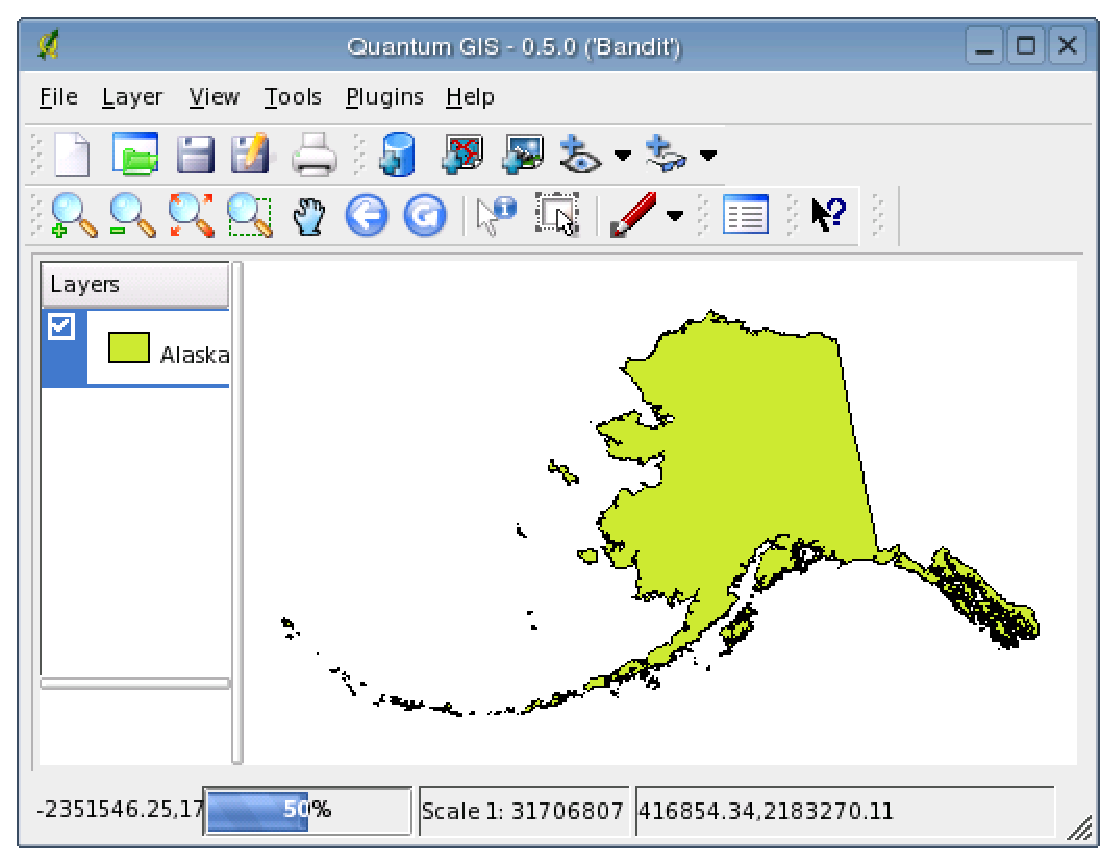
\includegraphics[scale=.7]{qgis_user_guide_images/shapefileloaded}
\end{center}  
   
\end{figure}
\begin{Tip}\caption{\textsc{Layer Colors}}
\qgistip{When you add a layer to the map, it is assigned a random color. When adding more than one layer at a time, different colors are assigned to each. }
\end{Tip}

Once loaded, you can zoom around the shapefile using the map navigation tools.
To change the symbology of a layer, open the layer properties dialog by double
clicking on the layer name or by right-clicking on the name in the legend and
choosing \textsl{Properties} from the popup menu. See Section
\ref{sec:symbology} for more information on setting symbology of vector
layers.  
\subsubsection{Improving Performance}
To improve the performance of drawing a shapefile, you can create a spatial
index. A \index{spatial index!shapefiles} spatial index will improve the draw speed when
zooming and panning.  

Use these steps to create the index:
\begin{compactenum}
\item Load a shapefile
\item Open the \textit{Layer Properties} dialog by double-clicking on the shapefile
name in the legend or by right-clicking and choosing \textit{Properties} from
the popup menu.
\item Click the \textit{Create} button on the Spatial Index panel
\end{compactenum}

\subsection{Loading a MapInfo Layer}
To load a MapInfo layer, click on the \textit{Add a vector layer}
toolbar bar button and change the file type filter to \textit{MapInfo (*.mif
*.tab *.MIF *.TAB)} and select the layer you want to load.

\subsection{Loading an ArcInfo Coverage}
Loading an an ArcInfo coverage is done using the same method as with a
shapefiles and MapInfo layers. Click on the \textit{Add a vector layer} toolbar
button to open the layer dialog.  Navigate to the coverage directory and select
one of the following files (if present in your coverage)
\begin{compactenum}
\item .lab - to load a label layer (polygon labels, or standing points
\item .cnt - to load a polygon centroid layer 
\item .arc - to load an arc (line) layer
\item .pal - to load a polygon layer
\end{compactenum}

\section{PostGIS Layers}\index{PostGIS!layers}
PostGIS layers are stored in a PostgreSQL database. The advantage of PostGIS
is the spatial indexing, filtering, and query capability. Using PostGIS,
vector functions such as select and identify work more accurately than with
OGR layers in QGIS.

To use PostGIS layers you must:\index{PostgreSQL!loading layers}
\begin{compactenum}
\item Create a stored connection in QGIS to the PostgreSQL database (if one is
not already defined)\index{PostgreSQL!connection}
\item Connect to the database
\item Select the layer to add to the map
\item Optionally provide a SQL \textit{where} clause to define which features to load from the layer
\item Load the layer
\end{compactenum}

\subsection{Creating a Stored Connection}\index{PostgreSQL!connection}
\parpic[l]{
\includegraphics{qgis_user_guide_images/addpostgis}}The first time
you use a PostGIS data source, you must create a connection to the PostgreSQL
database that contains the data. Begin by clicking on the \textit{Add a PostGIS
Layer} toolbar button. The \textsl{Add PostGIS Table(s)} dialog will be
displayed. To access the connection manager\index{PostgreSQL!connection
manager}, click on the \textsl{New} button to
display the \textsl{Create a New PostGIS Connection} dialog. The parameters
required for a connection are shown in Table \ref{tab:postgis_connection_parms}.

\begin{table}[h]\index{PostgreSQL!connection parameters}
\centering
\caption{PostGIS Connection Parameters}\label{tab:postgis_connection_parms}\medskip
 \begin{tabular}{|l|p{5in}|}
\hline Name & A name for this connection. Can be the same as \textsl{Database}
\\
\hline Host \index{PostgreSQL!host}
& Name of the database host. This must be a resolvable host name the same as would be used to open a telnet connection or ping the host \\
\hline Database \index{PostgreSQL!database} & Name of the database  \\
\hline Port \index{PostgreSQL!port}& Port number the PostgreSQL database server listens on. The default port is 5432.\\
\hline Username \index{PostgreSQL!username}& User name used to login to the database \\
\hline Password \index{PostgreSQL!password}& password used with \textsl{Username} to connect to the database\\
\hline
\end{tabular}
\end{table}
Once the parameters have been filled in, you can test the connection by clicking
on the \textsl{Test Connection} button\index{PostgreSQL!connection!testing}. To save the password with the connection information, check the \textsl{Save Password} option.
\begin{Tip}\caption{\textsc{QGIS User Settings and
Security}}\index{settings}\index{security}
\qgistip{Your customized settings for QGIS are stored based on the operating system. On Linux/Unix, the settings are stored in your home directory in .qt/qgisrc. On Windows, the settings are stored in the registry. Depending on your computing environment, storing passwords in your QGIS settings may be a security risk.
}
\end{Tip}
\subsection{Loading a PostGIS Layer}\index{PostgreSQL!loading layers}
\parpic[l]{
\includegraphics{qgis_user_guide_images/addpostgis}}Once you have one or more connections defined, you can load layers from the PostgreSQL database. Of course this requires having data in PostgreSQL. See Section \ref{sec:loading_postgis_data} for a discussion on importing data into the database. 

To load a layer from PostGIS, perform the following steps:
\begin{compactenum}
\item If the PostGIS layer dialog is not already open, click on the \textit{Add a PostGIS Layer} toolbar button
\item Choose the connection from the drop-down list and click \textsl{Connect}
\item Find the layer you wish to add in the list of available layers
\item Select it by clicking on it. You can select multiple layers by holding down the shift key while clicking. See Section \ref{sec:query_builder} for information on using the PostgreSQL Query Builder to further define the layer.
\item Click on the \textsl{Add} button to add the layer to the map
\end{compactenum}
\begin{Tip}\caption{\textsc{PostGIS Layers}}
\qgistip{Normally a PostGIS layer is defined by an entry in the geometry\_columns table. At version 0.7, QGIS can load layers that do not have an entry in the geometry\_columns table. This includes both tables and views. Defining a spatial view provides a powerful means to visualize your data.}
\end{Tip}
\subsection{Using the Query
Builder}\label{sec:query_builder}\index{PostgreSQL!query builder}
The PostgreSQL Query Builder allows you to define a subset of a table and add it
as a layer in QGIS.  For example, if you have a towns layer with a population
field you could select only larger towns by entering \textsl{population >
100000} in the SQL box of the query builder. Figure \ref{fig:querybuilder} shows an
example of the query builder populated with data from a layer in PostgreSQL. 

\begin{figure}[h]
  \begin{center}
    \caption{PostgreSQL Query Builder}\label{fig:query_builder}\smallskip
    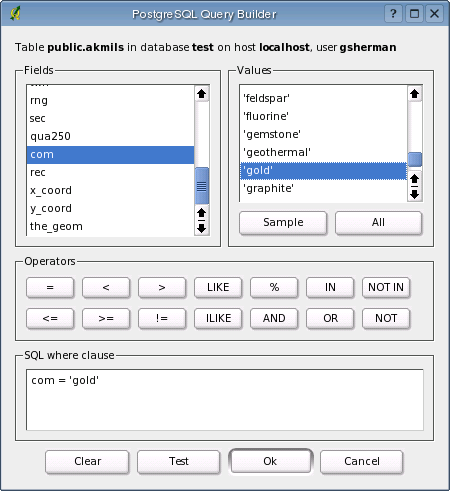
\includegraphics[scale=.6]{qgis_user_guide_images/querybuilder}
  \end{center}  
\end{figure}

The query builder\index{query builder} lists the layer's database
fields in the list box on the left.  You can get a sample of the data contained
in the highlighted field by clicking on the \textit{Sample} button\index{query
builder!generating sample list}. This
retrieves the first 25 distinct values for the field from the database. To get a
list of all possible values for a field, click on the \textit{All}
button\index{query builder!getting all values}. To
add a selected field or value to the query, double-click on it\index{query
builder!adding fields}. You can use the
various buttons to construct the query or you can just type it into the SQL box.

To test a query, click on the \textit{Test} button\index{query builder!testing
queries}. This will return a count of
the number of records that will be included in the layer. When satisfied with
the query, click \textit{Ok}. The SQL for the where clause will be shown in the
SQL column of the layer list.


\begin{Tip}\caption{\textsc{Changing the Layer Definition}}\index{query
builder!changing layer definitions}
\qgistip{You can change the layer definition after it is loaded by altering the
SQL query used to define the layer. To do this, open the vector layer properties
dialog by double-clicking on the layer in the legend and click on the
\textit{Query Builder} button on the \textit{General} tab. See Section
\ref{sec:vectorprops} for more information.}
\end{Tip}

\subsection{Some details about PostgreSQL layers}\label{sec:postgis_details}
\index{PostgreSQL!layer details}
This section contains some details on how QGIS accesses PostgreSQL
layers. Most of the time QGIS should simply provide you with a list of
database tables that can be loaded, and load them on request. However,
if you have trouble 
loading a PostgreSQL table into QGIS, the information below may help
you understand any QGIS messages and give you direction on changing
the PostgreSQL table or view definition to allow QGIS to load it.

QGIS requires that PostgreSQL layers contain a column that can be
used as a unique key for the layer. For tables this usually means
that the table needs a primary key, or have a column with a unique
constraint on it. QGIS additionally requires that this column be of
type int4 (an integer of size 4 bytes). If a table lacks these items,
the oid column will 
be used instead. Performance will be improved if the column is
indexed (note than primary keys are automatically indexed in PostgreSQL). 

If the PostgreSQL layer is a view the same requirements exist, but
views don't have primary keys or columns with unique constraints on
them. In this case QGIS will try to find a column in the view that is
derived from a table column that is suitable. If one cannot be found,
QGIS will not load the layer. If this occurs, the solution is to alter
the view so that it does include a suitable column (a type of int4
and either a primary key or with a unique constraint, preferably indexed).

\subsection{Importing Data into PostgreSQL}\label{sec:loading_postgis_data}
\index{SPIT!importing data}
Data can be imported into PostgreSQL using a number of methods. PostGIS
includes a utility called shp2pgsql that can be used to import shapefiles into
a PostGIS enabled database. For example, to import a shapefile named lakes into a PostgreSQL database named gis\_data, use the following command:
\begin{verbatim} 
  shp2pgsql -s 2964 lakes.shp lakes_new | psql gis_data
\end{verbatim}
This creates a new layer named lakes\_new in the the gis\_data database. The new layer will have a spatial reference identifier (SRID) of 2964. See Section \ref{sec:projections} for more information on spatial reference systems and projections.

\parpic[l]{
\includegraphics{qgis_user_guide_images/spiticon}}QGIS comes with a
plugin named SPIT (Shapefile to PostGIS Import Tool)\index{SPIT}.
SPIT can be used to load multiple shapefiles at one time and includes support
for schemas. To use SPIT, open the Plugin Manager from the Tools menu and load
the plugin by checking the box next to the SPIT plugin and click Ok. The SPIT
icon will be added to the plugin toolbar\index{SPIT!loading}. 

To import a shapefile, click on the SPIT tool in the toolbar to open the dialog.
You can add one or more files to the queue by clicking on the \textsl{Add}
button. To process the files, click on the Import button. The progress of the
import as well as any errors/warnings will be displayed as each shapefile is
processed.  
\begin{Tip}\caption{\textsc{Importing Shapefiles Containing
PostgreSQL Reserved Words}}\index{SPIT!reserved words}
\qgistip{If a shapefile is added to the queue containing fields that are
reserved words in the PostgreSQL database a dialog will popup showing the status
of each field. You can edit the field names\index{SPIT!editing field names}
prior to import and change any that are reserved words (or change any other
field names as desired). Attempting to
import a shapefile with reserved words as field names will likely fail.}
\end{Tip} 
\subsection{Improving Performance}
Retrieving features from a PostgreSQL database can be time consuming,
especially over a network. You can improve the drawing performance of
PostgreSQL layers by ensuring that a \index{spatial index!PostGIS} spatial index
exists on each layer in the database. PostGIS supports creation of a
\index{spatial index!GiST} GiST.
(Generalized Search Tree) index to speed up spatial searches of the data.

The syntax\footnote{GiST index information is taken from the PostGIS
documentation available at http://postgis.refractions.net} for creating a GiST index is:
\begin{verbatim}
    CREATE INDEX [indexname] ON [tablename] 
      USING GIST ( [geometryfield] GIST_GEOMETRY_OPS );
\end{verbatim}
Note that for large tables, creating the index can take a long time. Once the
index is created, you should perform a \textit{VACUUM ANALYZE}. See the
PostGIS documentation for more information.

The following is an example of creating a GiST index:
\begin{verbatim}
    gsherman@madison:~/current$ psql gis_data
    Welcome to psql 8.0.0, the PostgreSQL interactive terminal.

    Type:  \copyright for distribution terms
           \h for help with SQL commands
           \? for help with psql commands
           \g or terminate with semicolon to execute query
           \q to quit

    gis_data=# CREATE INDEX sidx_alaska_lakes ON alaska_lakes
    gis_data-# USING GIST (the_geom GIST_GEOMETRY_OPS);
    CREATE INDEX
    gis_data=# VACUUM ANALYZE alaska_lakes;
    VACUUM
    gis_data=# \q
    gsherman@madison:~/current$
\end{verbatim}
\section{The Vector Properties
Dialog}\label{sec:vectorprops}\index{vector layers!properties dialog} The
vector properties dialog provides information about a layer, symbology
settings, and labeling options. If your vector layer has been loaded from a
PostgreSQL / PostGIS datastore, you can also alter the underlying SQL for the
layer - either by hand editing the SQL on the \textit{General} tab, or by
invoking the query builder dialog on the \textit{General} tab. To access the
properties dialog, double-click on a layer in the legend or right-click on the
layer and select Properties from the popup menu.

\subsection{Vector Symbology}\label{sec:symbology}\index{vector
layers!symbology}

QGIS supports a number of symbology renderers to control how
vector features are displayed. Currently the following renderers
are available:

\begin{compactdesc}
    \item[Single symbol] - a single style is applied to every
    object in the layer.\index{vector layers!renderers!single symbol}
    \item[Graduated symbol] - objects within the layer are
    displayed with different symbols classified by the values of a
    particular field.\index{vector layers!renderers!graduated symbol}
    \item[Continuous colour] - objects within the layer are
    displayed with a spread of colours classified by the numerical
    values within a specified field.\index{vector layers!renderers!continuous color}
    \item[Unique value] - objects are classified by the unique
    values within a specified field with each value having a
    different symbol.\index{vector layers!renderers!unique value}
\end{compactdesc}

For layers containing point features, additional renderers are
available that use SVG icons:

\begin{compactdesc}
    \item[Single marker] - a single specified icon is used for
    every point within the layer.\index{vector layers!renderers!single marker}
    \item[Graduated marker] - points within the layer are
    displayed with different icons classified by values within a
    particular field.\index{vector layers!renderers!graduated marker}
    \item[Unique value marker] - points are classified by unique
    values within a specified field with each value having a
    different icon.\index{vector layers!renderers!unique value marker}
\end{compactdesc}

To change the symbology for a layer, simply double click on its legend entry and
the vector layer properties dialog will be shown.\index{symbology!changing}

\begin{figure}[h]
   \begin{center}
   \caption{Vector Layer Properties Dialog}\label{fig:vector_symbology}\smallskip
   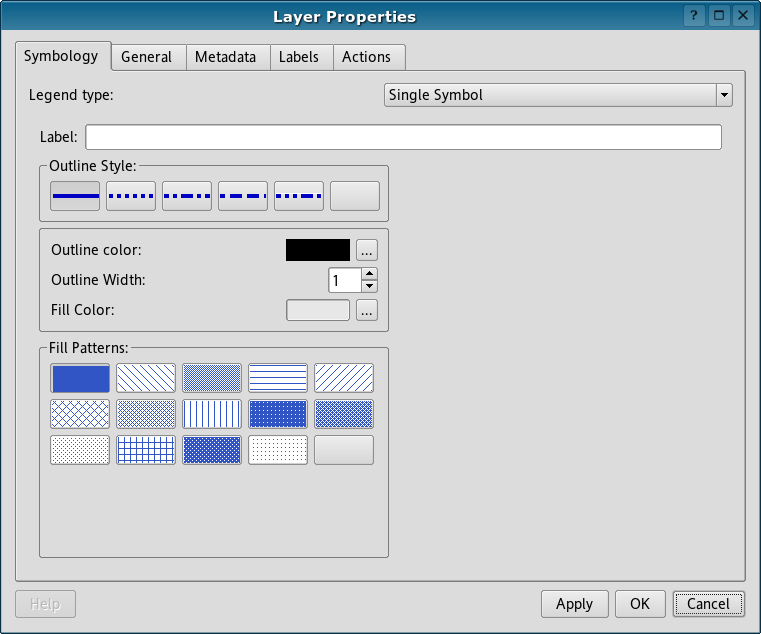
\includegraphics[scale=.5]{qgis_user_guide_images/vectorLayerSymbology}  
\end{center}  
\end{figure}
%force all figures to be printed
\section{Attribute Actions}\index{actions}
QGIS provides the ability to perform an action based on the attributes of a
feature. This can be used to perform any number of actions, for example,
running a program with arguments built from the attributes of a feature or
passing parameters to a web reporting tool.

Actions are useful when you frequently want to run an external application or
view a web page based on one or more values in your vector layer. An example is
performing a search based on an attribute value. This concept is used in the
following discussion.

\subsection{Defining Actions}\index{actions!defining}
Attribute actions are defined from the vector layer properties dialog. To define
an action, open the vector layer properties dialog and click on the
\textit{Actions} tab. Provide a descriptive name for the action. The action
itself must contain the name of the application that will be executed when the
action is invoked. You can add one or more attribute field values as arguments
to the application. When the action is invoked any set of characters that start
with a \% followed by the name of a field will be replaced by the value of that
field.  The special characters \%\% \index{\%\%}will be replaced by the value of
the field that was selected from the identify results or attribute table (see
Using Actions below).  Double quote marks can be used to group text into a
single argument to the program, script or command. Double quotes will be ignored
if proceeded by a backslash.  

Two example actions are shown below:\index{actions!examples}
\begin{compactenum}
  \item \texttt{konqueror http://www.google.com/search?q=\%nam}
  \item \texttt{konqueror http://www.google.com/search?q=\%\%}
\end{compactenum}
In the first example, the web browser konqueror is invoked and passed a URL to
open. The URL performs a Google search on the value of the \textit{nam} field
from our vector layer. Note that the application or script called by the action
must be in the path or you must provided the full path. To be sure, we could
rewrite the first example as: \texttt{/opt/kde3/bin/konqueror
http://www.google.com/search?q=\%nam}. This will ensure that the konqueror
application will be executed when the action is invoked.

The second example uses the \%\% notation which does not rely on a particular
field for its value. When the action is invoked, the \%\% will be replaced by
the value of the selected field in the identify results or attribute table.

\subsection{Using Actions}\index{actions!using}
Actions can be invoked from either the \textit{Identify Results} dialog or the
\textit{Attribute table} dialog. To invoke an action, right click on the record
and choose the action from the popup menu. Actions are listed in the popup menu
by the name you assigned when defining the actions. Click on the action you wish
to invoke.

If you are invoking an action that uses the \%\% notation, right-click on the
field value in the \textit{Identify Results} dialog or the
\textit{Attribute table} that you wish to pass to the application or script.

Here is another example that pulls data out of a vector layer and inserts it
into a file using bash and the `echo' command (so it will only work on Gnu/Linux
and perhaps Mac OS X). The layer in question has fields for a species name
(taxon\_name), latitude (lat) and longitude (long). I would like to be able to
make a spatial selection of a localities and export these field values to a text
file for the selected record (shown in yellow in the QGIS map area). Here is the
action to achieve this:

\begin{verbatim}
	bash -c "echo \"%taxon_name %lat %long\" >> /tmp/species_localities.txt"
\end{verbatim} 

After selecting a few localities and running the action on each one, opening the output file will show something like this:

\begin{verbatim}
	Acacia mearnsii -34.0800000000 150.0800000000
	Acacia mearnsii -34.9000000000 150.1200000000
	Acacia mearnsii -35.2200000000 149.9300000000
	Acacia mearnsii -32.2700000000 150.4100000000
\end{verbatim} 


\section{Editing}\index{editing}

QGIS supports basic capabilities for editing spatial data.  Before reading any
further you should note that at this stage editing support is still preliminary.
Before performing any edits, always make a backup of the dataset you are about
to edit. 

\textbf{Note} - the procedure for editing GRASS layers is different - see
Section \ref{grass_digitising} for details.

\subsection{Editing an Existing Layer}\index{editing!an existing layer}
\label{sec:edit_existing_layer}
If you wish to edit an existing layer, choose \textit{Start Editing} from the
context menu after right clicking on the legend entry for that layer. Remember
to backup your data before starting! Once the layer is in edit mode you will
see a small 
\includegraphics[scale=1]{qgis_user_guide_images/editable} icon to
remind you.\index{editing!icon}

Now that the layer is editable, you can use the \textit{Capture Points} icon (or
similar icon for line and polygon layers) on the toolbar to put the QGIS cursor
into digitising mode. If you are capturing a point feature simply use the pan
and zoom tools to navigate to the area of interest, then click the
\textit{Capture Points} tool and click on the map area to create the  
new point feature. A window will appear allowing you to set the attributes.
Figure \ref{fig:vector_digitising} shows setting attributes for a fictitious
new city in the Antarctic.

\begin{figure}[h]
   \begin{center}
   \caption{Vector Digitizing Attributes Capture Dialog}\label{fig:vector_digitising}\smallskip
   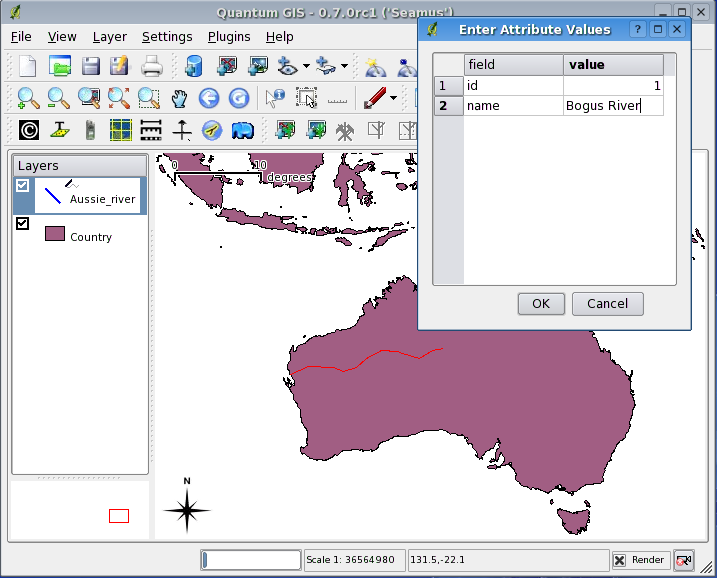
\includegraphics[scale=.65]{qgis_user_guide_images/digitising_attributes}
\end{center}  
\end{figure}

In its current implementation the attributes dialog box does not check that the
data matches the type expected, so make sure of this before
pressing \textit{Ok}. 

To delete a feature, select it using the selection tool and choose
\textit{Delete selection} from the editing tools.

Once you have finished adding features, choose \textit{Stop Editing} from the
layer's context menu. Choosing \textit{Yes} will save the changes to disk, while
choosing \textit{No} at this point will cause them to be discarded.
\index{editing!saving changes}
%Note that QGIS does not yet provide any way to delete an individual feature.

\subsection{Creating a New Layer}\index{editing!creating a new layer}

To create a new layer for editing, choose \textit{New Vector Layer} from the
\textit{Layer} menu. The \textit{New Vector Layer} dialog will be displayed as
shown in Figure \ref{fig:newvectorlayer}. Choose the type of layer (point,
line, or polygon). 
\begin{figure}[h]
   \begin{center}
   \caption{Creating a New Vector Dialog}\label{fig:newvectorlayer}\smallskip
   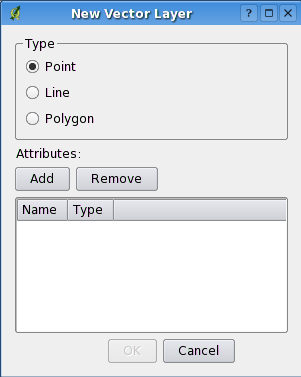
\includegraphics[scale=.75]{qgis_user_guide_images/newvectorlayer}
\end{center}  
Note that QGIS does not yet support creation of 2.5D
features (i.e. features with X,Y,Z coordinates) or measure features. At this
time, only shapefiles can be created. In a future version of QGIS, creation of
any OGR or PostgreSQL layer type will be supported.

\end{figure}
To complete the creation of the new layer, add the desired attributes by
clicking on the \textit{Add} button and specifying a name and type for the
attribute. Only real, integer, and string attributes are supported. Once you
are happy with the attributes, click Ok and provide a name for the shapefile.
QGIS will automatically add a .shp extension to the name you specify.  Once
the layer has been created, it will be added to the map and you can edit it in
the same way as described in Section \ref{sec:edit_existing_layer} above. 
 not translated yet
%\chapter{Working with Raster Data}
QGIS supports a number of raster data formats. This section describes how to work with raster data in QGIS.
\section{What is raster data?}
index{rasters!definition}
Raster data in GIS are matrices of discrete cells that represent features on, above or below the earth's surface. Each cell in the raster grid is the same size, and cells are usually rectangular (in QGIS they will always be rectangular). Typical raster datasets include remote sensing data such as aerial photography or satellite imagery and modelled data such as an elevation matrix.

Unlike vector data, raster data typically do not have an associated database record for each cell.

In GIS, a raster layer would have georeferencing data associated with it which
will allow it to be positioned correctly in the map display to allow other
vector and raster data to be overlaid with it. QGIS makes use of georeferenced
rasters to properly display the data.\index{rasters!georeferenced}
	
\section{Raster formats supported in QGIS}
QGIS supports a number of different raster formats. Currently tested formats
include:\index{rasters!formats}
\begin{compactitem}
\item Arc/Info Binary Grid
\item Arc/Info ASCII Grid
\item Grass Raster
\item GeoTIFF
\item Spatial Data Transfer Standard Grids (with some limitations)
\item USGS ASCII DEM
\item Erdas Imagine
\end{compactitem}
Because the raster implementation in QGIS is based on the GDAL library, other
raster formats implemented in GDAL are also likely to work, but have not yet
been tested. See Appendix \ref{appdx_gdal} for more
details.\index{rasters!implementation}
	
\section{Loading raster data in QGIS}
\parpic[l]{
\includegraphics{qgis_user_guide_images/addraster}}Raster layers are
loaded either by clicking on the Load Raster icon or by selecting the View->Add
Raster Layer menu option. More than one layer can be loaded at the same time by
holding down the Control key and clicking on multiple items in the file
dialog.\index{rasters!loading}
	
\section{Raster Properties}

\parpic[r]{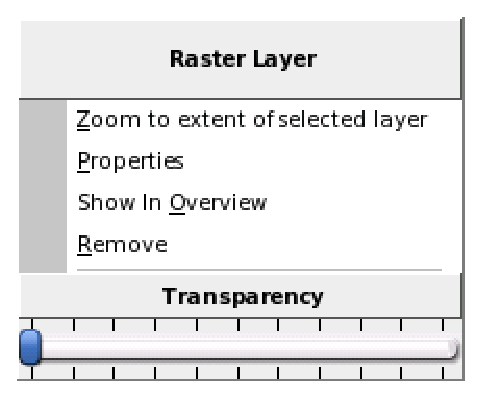
\includegraphics[scale=0.6]{qgis_user_guide_images/rastercontextmenu}}To
view and set the properties for a raster layer, right click on the layer name.
This displays the raster layer context menu that includes a number of items that
allow you to:\index{rasters!context menu}
\begin{compactitem}
\item Zoom to the full extent of the raster
\item Show the raster in the map overview window
\item Open the properties dialog (of course)
\item Remove the layer from the map
\item Set the transparency using a slider control
\end{compactitem}
Choose \textsl{Properties} from the context menu to open the raster properties
dialog for the layer.\index{rasters!properties}


Figure \ref{fig:raster_properties} shows the properties dialog. There are four tabs on the dialog: \textsl{Symbology}, \textsl{General}, \textsl{Metadata}, and \textsl{Pyramids}.

\begin{figure}[h]
   \begin{center}
   \caption{Raster Layers Properties Dialog}\label{fig:raster_properties}\smallskip
   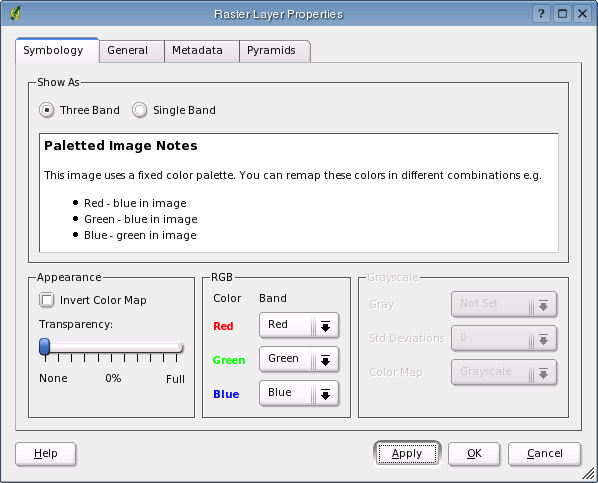
\includegraphics[scale=.7]{qgis_user_guide_images/raster_properties}
\end{center}  
\end{figure}


\subsection{Symbology Tab}


QGIS supports three forms of raster layers:\index{rasters!supported forms}
\begin{compactitem}
\item Single Band Grayscale Rasters
\item Palette Based RGB Rasters
\item Multiband RGB Rasters
\end{compactitem}

From these three basic layer types, eight forms of symbolised raster display can
be used:\index{rasters!renderers}
\begin{compactenum}

\item Single Band Grayscale
\item Single Band Pseudocolor
\item Paletted Grayscale (where only the red, green or blue component of the image is displayed)
\item Paletted Pseudocolor (where only the red, green or blue component of the image is displayed, but using a pseudocolor algorithm)
\item Paletted RGB
\item Multiband Grayscale (using only one of the bands to display the image)
\item Mulitiband Pseudocolor (using only one of the bands shown in pseudocolor)
\item Multiband RGB (using any combination of three bands)
\end{compactenum}
\smallskip
QGIS can invert the colors in a given layer so that light colors become dark
(and dark colors become light). Use the \textsl{Invert Color Map} checkbox to
enable / disable this behavior.\index{rasters!inverting the color map}

QGIS has the ability to display each raster layer at varying transparency
levels.\index{rasters!transparency} Use the transparency slider to indicate to what extent the underlying layers (if any) should be visible though the current raster layer. The transparency can also be set using the transparency slider in the layer context menu which is accessible by right-clicking on the layer in the legend.

QGIS can restrict the data displayed to only show cells whose values are within
a given number of standard deviations of the mean for the
layer.\index{rasters!standard deviation} This is useful when you have one or two cells with abnormally high values in a raster grid that are having a negative impact on the rendering of the raster. This option is only available for pseudocolor images.

\subsection{General Tab}
The General tab displays basic information about the selected raster, including
the layer source and  display name in the legend (which can be modified). This
tab also shows a thumbnail of the layer, its legend symbol, and the
palette.\index{rasters!properties}

\subsection{Metadata Tab}
The Metadata tab displays a wealth of information about the raster layer,
including statistics about each band in the current raster layer. Statistics are
gathered on a 'need to know' basis, so it may well be that a given layers
statistics have not yet been collected.\index{rasters!metadata}


\begin{Tip}\caption{\textsc{Gathering Raster Statistics}}
\qgistip{To gather statistics for a layer, select pseudocolor rendering and
click the \textsl{Apply} button. Gathering statistics for a layer can be time
consuming. Please be patient while QGIS examines your
data!\index{rasters!statistics}
}
\end{Tip}
\subsection{Pyramids Tab}
\label{raster_pyramids}
Large resolution raster layers can slow navigation in QGIS. By creating lower
resolution copies of the data (pyramids), performance can be considerably
improved as QGIS selects the most suitable resolution to use depending on the
level of zoom.\index{rasters!building pyramids} 

You must have write access in the directory where the original data is stored to build pyramids. 

Please note that building pyramids may alter the original data file and once created they cannot be removed. If you wish to preserve a 'non-pyramided' version of your raster, make a backup copy prior to building pyramids.
 not translated yet
%% vim:autoindent:set textwidth=78:
\chapter{Working with Projections}
QGIS supports on the fly projection of vector layers. This feature allows you
to display layers with different coordinate systems and have them overlay
properly. 
\section{Overview of Projection Support}
QGIS has support for approximately 2,700 known projections. 
Projections are stored in a Sqlite database that is installed with QGIS.
Appendix \ref{app:datamodel}  contains information about the database and the
schema. Normally you do not need to manipulate the database directly. In fact,
doing so may cause projection support to fail. Custom projections are
stored in a user database. See Section \ref{sec:custom_projections} for
information on managing your custom projections.

The projections available in QGIS are based on those defined by EPSG and are
largely abstracted from the spatial\_references table in PostGIS version 1.x.
Note that the identifiers used in QGIS do not correspond to the EPSG or
PostGIS spatial reference identifiers. The EPSG and PostGIS identifiers are
present in the database and can be used to specify a projection in QGIS.

In order to use OTF projection, your data must contain information about its
coordinate system. For PostGIS layers QGIS uses the spatial reference
identifier that was specified when the layer was created. For data supported
by OGR, QGIS relies on the presence of a format specific means of specifying
the coordinate system. In the case of shapefiles, this means a file containing
the Well Known Text (WKT) specification of the the coordinate system. The
projection file has the same base name as the shapefile and a prj extension.
For example, a shapefile named lakes.shp would have a corresponding projection
file named lakes.prj.


%\section{Requirements}
%QGIS uses the Proj4 to provide projection support. 
\section{Getting Started}
At startup, QGIS does not have On-the-Fly (OTF) projection enabled. To use OTF
projection, you must open the \textit{Project Properties} dialog, select a
projection for the map,  and enable projections.  There are two ways to open
the \textit{Project Properties} dialog:
\begin{compactenum}
\item Select \textit{Project Properties} from the \textit{Settings} menu
\item Click on the projector icon in the lower right-hand corner of the
statusbar
\end{compactenum}
\begin{Tip}
 \caption{\textsc{Project Properties Dialog}}
\qgistip{
If you open the \textit{Project Properties} dialog from the Settings menu, you must
click on the \textit{Projection} tab to view the projection settings. Opening
the dialog from the projector icon will automatically bring the
\textit{Projection} tab to the front.
}
\end{Tip}
The Projection dialog contains four important components as numbered in Figure
\ref{fig:projections} and described below.
\begin{figure}[h]
   \begin{center}
   \caption{Projection Dialog (OS X)}\label{fig:projections}\smallskip
   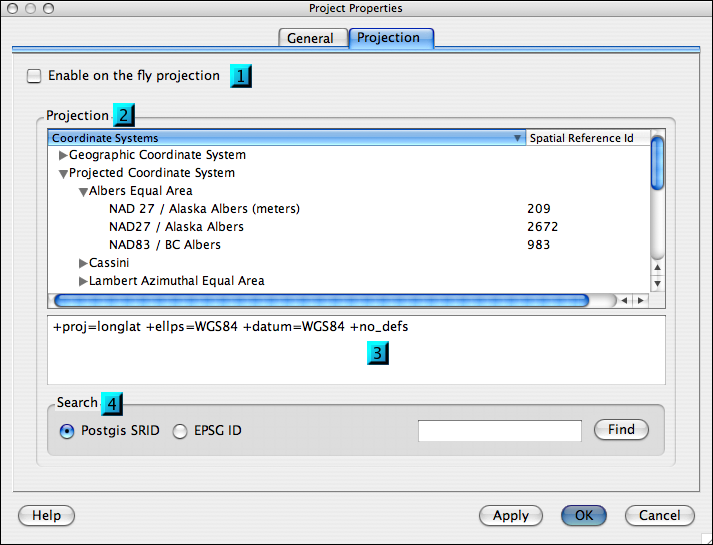
\includegraphics[scale=.70]{qgis_user_guide_images/projectiondialog}
\end{center}  
\end{figure}
\begin{compactenum}
\item Enable projections - this checkbox is used to enable or disable OTF
projection. When off, no projection takes place and each layer
is drawn using the coordinates as read from the data source. When on, the
coordinates in each layer are projected to the coordinate system of the map
canvas.
\item Projections - this is a list of all projection supported by QGIS,
including Geographic, Projected, and Custom coordinate systems. To use a
coordinate system, select it from the list by expanding the appropriate node
and selecting the projection.
\item Proj4 text - this is the projection string used by the Proj4 projection
engine. This text is read-only and provided for informational purposes.
\item Search - if you know the PostGIS or EPSG identifier for a projection,
you can use the search feature to find it. Enter the identifier and click on
\textit{Find}.

\end{compactenum}
\subsection{Specifying a Projection}
QGIS automatically sets the map projection to the coordinate system of the first
layer loaded. One way to specify the map projection is to first load a layer
with the projection you want for the entire map. Then open the \textit{Project Properties} 
dialog and click on the \textit{Enable on the fly projection} checkbox. You
can now close the \textit{Project Properties} dialog and add additional layers
to the map. 

If you have already added layers and want to enable OTF projection, open the 
\textit{Project Properties} dialog and find the projection or geographic
coordinate system you want to use in the list of projections. Alternatively
you can use the search feature as described in the previous section.

\section{Custom Projections}
If QGIS doesn't have the projection you need, you can define a custom
projection. 
 not translated yet
%\chapter{GRASS}\label{sec:grass}\index{GRASS}
The GRASS plugin adds the following features to QGIS:
\begin{compactitem}
\item Add GRASS vector layers
\item Add GRASS raster layers
\item Vector layers digitizing
\item Changing of the GRASS region
\end{compactitem}
\section{Starting QGIS with
GRASS}\label{sec:starting_grass}\index{GRASS!starting QGIS}
When using the GRASS plugin, QGIS can be started in two ways: from the GRASS shell or from a regular shell.
\subsection{From GRASS shell}

If QGIS is started from the GRASS shell (GRASS started by grass57 command), no
additional settings are required. \index{GRASS!shell}
\subsection{Outside GRASS shell}

If QGIS is not started from the GRASS shell, the environment variables must be properly set before starting QGIS.
 
The path to GRASS libraries must be added to LD\_LIBRARY\_PATH environment
variable. For example (in bash): \index{GRASS!environment settings}
\begin{verbatim}
    export LD_LIBRARY_PATH=/usr1/grass57/dist.i686-pc-linux-gnu/lib:$LD_LIBRARY_PATH
\end{verbatim}    
 
The GISBASE environment variable must be set to the full path of the directory where GRASS is installed (the same as used for --with-grass= option). For example (in bash):
\begin{verbatim}
    export GISBASE=/usr1/grass57/dist.i686-pc-linux-gnu 
\end{verbatim}
\section{Loading GRASS Data}\index{GRASS!loading data}
With the GRASS plugin loaded, you can load a vector or raster layer using the appropriate button on the toolbar. \begin{Tip}\caption{\textsc{GRASS Data Loading}}
\qgistip{If you have problems loading data or QGIS terminates abnormally, check to make sure you have started GRASS properly as described in Section \ref{sec:starting_grass}.
}
\end{Tip} 
\section{Vector Data Model}\index{GRASS!vector data model}
It is important to understand the GRASS vector data model prior to
digitizing.\index{GRASS!digitizing}
In general, GRASS uses a topological vector model.\index{GRASS!topology} This
means that areas are not represented as closed polygons, but by one or more
boundaries. A boundary between two adjacent areas is digitized only once, and it
is shared by both areas. Boundaries must be connected without gaps. An area is
identified (labeled) by the centroid of the area.

Besides boundaries and centroids, a vector map can also contain
points and lines. All these geometry elements can be mixed
in one vector.

It is possible to store more 'layers' in one vector dataset. For example,
fields, forests and lakes can be stored in one vector. Adjacent
forest and lake can share the same boundary, but they have separate attribute tables.
It is also possible to attach attributes to boundaries. For example, the boundary between lake and forest is a road with different attribute table.
%In addition, one geometry element can represent a geometry for more
%features. For example, a road can be a marked turistic route at the same 
%time.

The 'layer' of the feature is defined by 'field' (sorry for this name).
'Field' is the number which defines if the geometry is forest or lake.
For now, it can be only a number, in the future GRASS will also support  
names as fields in the user interface.

Attributes are stored in external database tables, for example
DBF, PostgreSQL, etc.\index{GRASS!attribute storage}

Attributes in database tables are linked to geometry elements
using 'category'.\index{GRASS!attribute linkage} 'Category' (key, ID) is an
integer attached to geometry primitives, and it is used as the link to one
column in the database table.
\begin{Tip}\caption{\textsc{Learning the GRASS Vector Model}}
\qgistip{The best way to learn the GRASS vector model and its capabilities
is to download the demo mapset from \url{http://mpa.itc.it/radim/g51/g51test-12-multi.tar.gz}.
Extract the mapset, add all layers from vector 'multi' to QGIS, and query attributes.
Finaly start editing of vector 'multi', to see how those layers are stored.
}
\end{Tip} 
\section{Digitizing and Editing Tools}\index{GRASS!digitizing tools}
\label{grass_digitising}
The digitizing tools for GRASS vector layers are accessed using the \textsl{Edit GRASS Vector Layer} tool on the toolbar. Make sure you have loaded a GRASS vector and it is the selected layer in the legend before clicking on the edit tool. In this release, the vector must exist prior to beginning to edit. The ability to create a new "empty" layer will be added in a future version. Figure \ref{fig:grass_edit} shows the GRASS Edit dialog that is displayed when you click on the edit tool. 
\begin{figure}[h]
   \begin{center}
   \caption{GRASS Edit Dialog}\label{fig:grass_edit}\smallskip
   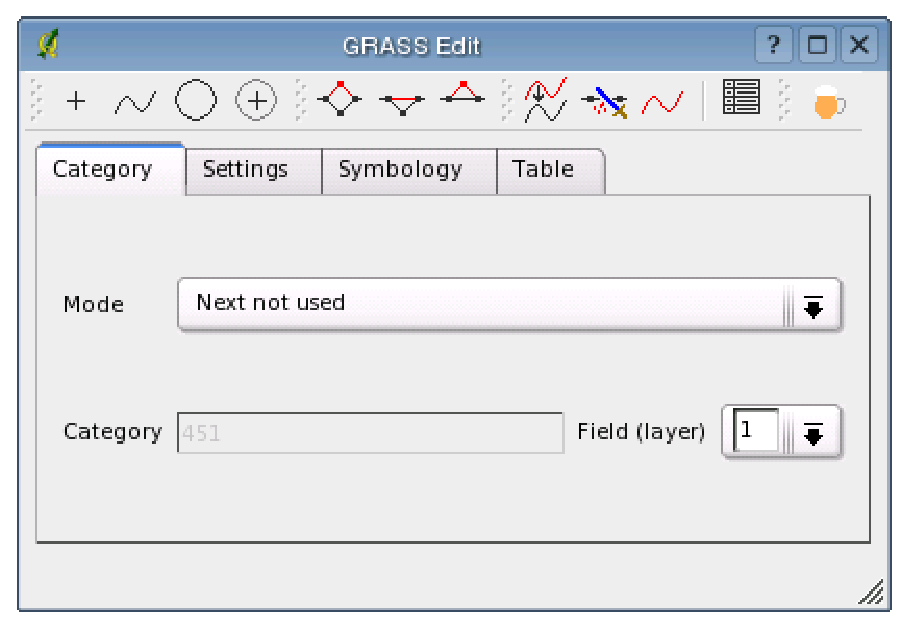
\includegraphics[scale=.7]{qgis_user_guide_images/grassedit}
\end{center}  
\end{figure}
The tools and settings are discussed in the following sections.
\subsection{Toolbar}
Table \ref{tab:grass_tools} lists the digitizing tools provided by the GRASS plugin. These correspond to the tool buttons in the toolbar(s) across the top of the dialog.
\begin{table}[h]\index{GRASS!digitizing tools}

\centering
\caption{GRASS Digitizing Tools}\label{tab:grass_tools}\medskip
 \begin{tabular}{|l|p{5in}|}
 \hline \textbf{Tool} & \textbf{Purpose} \\
\hline New Point & digitize new point \\
\hline New Line &  digitize new line (finish by selecting new tool) \\
\hline New Boundary & digitize new boundary (finish by selecting new tool)\\
\hline New Centroid & digitize new centroid (label existing area)\\
\hline Move vertex & select one vertex of existing line or boundary and identify new position\\
\hline Add vertex & add a new vertex to existing line\\
\hline Delete vertex & delete one vertex from existing line (confirm selected vertex by another click)\\
\hline Move line & select existing line and click on new position\\
\hline Split line & split an existing line to 2 parts\\
\hline Delete line & delete existing line (confirm selected line by another click)\\
\hline Edit attributes & edit attributes of existing element (note that one element can represent more features, see above)\\
\hline Mug & close digitizing session\\
\hline
\end{tabular}
\end{table}
\subsection{Category Tab}\index{GRASS!category settings}
This tab allows you to set the way in which the category will be assigned to each new feature and/or assign a category to a feature.
\begin{compactitem}
\item Mode: what category should be attached to geometry
\begin{compactitem}
\item Next not used - next category not yet used in vector
\item Manual entry - define the category in 'Category entry'
\item No category - digitize geometry without category
\end{compactitem}
\item Category - a number (ID) attached to digitized feature
\item Field - feature (attribute table) identification
\end{compactitem}
\subsection{Settings Tab} \index{GRASS!snapping tolerance}
This tab allow you to set the snapping in screen pixels. This is the threshold in pixels in which new points or line ends are snapped to existing nodes. This helps prevent gaps or dangles between boundaries

\subsection{Symbology Tab}\index{GRASS!symbology settings}
This tab allows you to view and set symbology for various geometry types and their topological status (e.g. closed / opened boundary).

\subsection{Table} \index{GRASS!table editing}
This tab provides the means to view, create, or modify the database table for a given field.
\begin{Tip}\caption{\textsc{GRASS Edit Permissions}}\index{GRASS!edit permissions}
\qgistip{You must be the owner of the GRASS mapset you want to edit. It is impossible to edit vectors in mapsets which are not yours, even if you have write permissions.
}
\end{Tip} 

\subsection{Region Tool}\index{GRASS!region}

The current region (window) in GRASS is very important for all 
raster modules. All new created rasters have the extension and resolution
of the current region, regardless their original region. 
The region is stored in \$LOCATION/\$MAPSET/WIND file, and it defines
north, south, east, west, number of columns, number of rows, 
horizontal and vertical resolution.

It is possible to switch on/off the grass region in QGIS canvas
using the \textsl{Display Current GRASS Region}
button. \index{GRASS!region!display}

With the \textsl{Edit Current GRASS Region} you can open a tool 
in which you can change the current region and symbology
of the rectangle on the QGIS Canvas. When the tool is running,
it is also possible to select a new region interactively
on the QGIS canvas.\index{GRASS!region!editing}

Both tools are available only if QGIS was started from a GRASS 
shell or if the GISRC enviroment variable pointing to a
valid GISRC file was set (i.e. only if you are running 
GRASS within your mapset).

%\section{The GRASS Toolbar}
%The GRASS toolbar is displayed when the GRASS plugin is loaded using the Plugin Manager (see Section \ref{sec:managing_plugins}, \textsl{Managing Plugins}). Figure  shows the toolbar with each function annotated.
 not translated yet
%first the general intro to plugins
%then each individual plugin can have a section
%in the plugins chapter
%\chapter{Using Plugins}\index{plugins}
\section{An Introduction to Using Plugins}
QGIS has been designed with a plugin architecture. This allows new features/functions to be added to the application. Many of the features in QGIS are actually implemented as plugins.

There are two types of plugins in QGIS: core and user-contributed.
\index{plugins!types}A core plugin is maintained by the QGIS development team and is part of every QGIS distribution. A user-contributed plugin is an external plugin that is maintained by the individual author. The QGIS Community site (\url{http://community.qgis.org}) serves as the repository for user contributed plugins.

\subsection{Finding and Installing a Plugin}
When you install QGIS, all of the core plugins are included (these are described
below). \index{plugins!installing}Additional user-contributed plugins may be
available on the QGIS Community site. To see what user-contributed plugins are
available, see the plugins page on the Community site
(\url{http://community.qgis.org/plugins}).\index{plugins!user contributed}

Typically user-contributed plugins are distributed in source form and require compiling. For instructions on building and installing a user-contributed plugin, see the documentation included with the plugin.
\subsection{Managing Plugins}\label{sec:managing_plugins}\index{plugins!managing}
Managing plugins consists of loading or unloading them from QGIS. Loaded plugins are "remembered" when you exit the application and restored the next time you run QGIS.

To manage plugins, open the \textsl{Plugin Manager} from the \textsl{Tools}
menu. \index{plugins!manager}The Plugin Manager displays all the available plugins and their status (loaded or unloaded). Figure \ref{fig:pluginmanager} shows the Plugin Manager dialog.

\begin{figure}[h]
   \begin{center}
   \caption{Plugin Manager}\label{fig:pluginmanager}\smallskip
   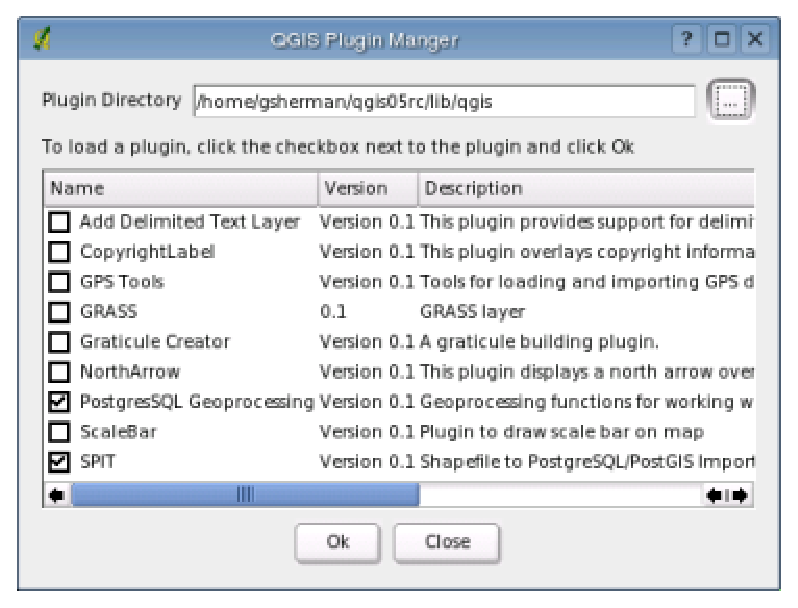
\includegraphics{qgis_user_guide_images/pluginmanager_80pct}
\end{center}  
\end{figure}
Typically all QGIS plugins are installed in the same location. This location is shown in the Plugin Directory text field. You can tell QGIS to load plugins from another location by specifying a different directory.
\begin{Tip}\caption{\textsc{Crashing Plugins}}\index{crashes}
\qgistip{If you find that QGIS crashes on startup, a plugin may be at fault. You can stop all plugins from loading by editing your .qt/qgisrc file in your home directory on Linux/Unix (Windows users will have to edit the registry). On Linux/Unix, open the qgisrc file in a text editor and find the [Plugins] section. Set all the plugin values to false to prevent them from loading. For example, to prevent the Delimited text plugin from loading, the entry in qgisrc should look like this:\ttfamily{
 Add Delimited Text Layer=false}.\normalfont  Do this for each plugin in the [Plugins] section. You can then start QGIS and add the plugins one at a time from the Plugin Manger to determine which is causing the problem.

}
\end{Tip} 

\subsection{Data Providers}\index{data providers}
Data Providers are "special" plugins that provides access to a data store. By default, QGIS supports PostGIS layers and disk-based data stores supported by the OGR library (Appendix \ref{appdx_ogr}). A Data Provider plugin extends the ability of QGIS to use other data sources.

Data Provider plugins are registered automatically by QGIS at startup. They are not managed by the Plugin Manager but are used behind the scenes when a corresponding data type is added as a layer in QGIS.
\subsection{Core Plugins}\index{plugins!core}
QGIS currently contains 9 core plugins that can be loaded using the Plugin Manager. Table \ref{tab:core_plugins} lists each of the core plugins along with a description of their purpose. Figure \ref{fig:plugintoolbar} shows the icon for each plugin in the Plugin toolbar (the number corresponds to the Item in Table \ref{tab:core_plugins}. Note the GRASS plugin is not included below because it installs its own toolbar (see Section \ref{sec:grass} for a discussion of available features in GRASS plugin).
\begin{table}[h]
\centering
\caption{QGIS Core Plugins}\label{tab:core_plugins}\medskip
\small
 \begin{tabular}{|l|l|p{4in}|}
\hline \textbf{Item} & \textbf{Plugin} & \textbf{Description} \\
\hline 1 & Copyright Label \index{plugins!copyright}& Display a copyright label on the map canvas\\
\hline 2 & Delimited Text \index{plugins!delimited text}& Load a delimited text file containing x,y coordinates as a point layer \\
\hline 3 & GPS Tools \index{plugins!gps}& Load and display GPS data \\
\hline 4 & Graticule Creator \index{plugins!graticule}& Create a latitude/longitude grid and save as a shapefile\\
\hline 5 & Scalebar \index{plugins!scalebar}& Add a scalebar to the map canvas\\
\hline 6 & North Arrow \index{plugins!north arrow}& Add a north arrow to the map canvas\\
\hline 7 & PostgreSQL Geoprocessing \index{plugins!geoprocessing}& Buffer a PostGIS layer \\
\hline 8 & SPIT \index{plugins!SPIT}& Shapefile to PostGIS Import Tool - import shapefiles into PostgreSQL\\
\hline
\end{tabular}
\end{table}
\normalsize
\begin{figure}[h]
   \begin{center}
   \caption{Plugin Toolbar and Icons}\label{fig:plugintoolbar}\smallskip
   
\includegraphics[scale=1.0]{qgis_user_guide_images/plugintoolbar}
\end{center}  
\end{figure}

\begin{Tip}\caption{\textsc{Plugins Settings Saved to Project}}\index{plugins settings}
\qgistip{When you save a .qgs project, any changes you have made to NorthArrow, ScaleBar and Copyright plugins will be saved in the project and restored next time you load it.
}
\end{Tip}
 not translated yet
%\section{Using the GPS Plugin}


\subsection{What is GPS?}

GPS, the Global Positioning System, is a satellite-based system that
allows anyone with a GPS receiver to find their exact position anywhere
in the world. It is used as an aid in navigation, for example in airplanes,
in boats, and by hikers. The GPS receiver uses the signals from the
satellites to calculate its latitude, longitude and (sometimes) elevation.
Most receivers also have the capability to store locations (known
as \emph{waypoints}), sequences of locations that make up a planned
\emph{route}, and a tracklog or \emph{track} of the receivers movement
over time. Waypoints, routes, and tracks are the three basic feature
types in GPS data. QGIS displays waypoints in point layers while routes
and tracks are displayed in linestring layers.


\subsection{Loading GPS data from a file}

There are dozens of different file formats for storing GPS data. The
format that QGIS uses is called GPX (GPS eXchange format), which is
a standard interchange format that can contain any number of waypoints,
routes, and tracks in the same file.

\includegraphics{qgis_user_guide_images/plugins_gps/icon}To load a GPX file you need to use the \emph{GPS Tools} plugin. When
this plugin is loaded a button with a small handheld GPS device will
show up in the toolbar (the device looks a bit like a mobile phone).
Clicking on this button will open the \emph{GPS Tools} dialog (see
figure \ref{figure GPX loader}).

%
\begin{figure}

\caption{\label{figure GPX loader}The \emph{GPS Tools} dialog window}

\includegraphics[%
  scale=0.5]{qgis_user_guide_images/plugins_gps/loadgpx}
\end{figure}


Use the browse button {[}...{]} to select the GPX file, then use the
checkboxes to select the feature types you want to load from that
GPX file. Each feature type will be loaded in a separate layer when
you click OK.


\subsection{GPSBabel}

Since QGIS uses GPX files you need a way to convert other GPS file
formats to GPX. This can be done for many formats using the free program
GPSBabel, which is available at \url{http://www.gpsbabel.org}. This
program can also transfer GPS data between your computer and a GPS
device. QGIS uses GPSBabel to do these things, so it is recommended
that you install it. However, if you just want to load GPS data from
GPX files you will not need it. Version 1.2.3 of GPSBabel is known
to work with QGIS, but you should be able to use later versions without
any problems.


\subsection{Importing GPS data}

To import GPS data from a file that is not a GPX file, you use the
tool \emph{Import other file} in the \emph{GPS Tools} dialog. Here
you select the file that you want to import, which feature type you
want to import from it, where you want to store the converted GPX
file, and what the name of the new layer should be.

When you select the file to import you must also select the format
of that file by using the menu in the file selection dialog (see figure
\ref{figure importdialog}). All formats do not support all three
feature types, so for many formats you will only be able to choose
between one or two types.

%
\begin{figure}

\caption{\label{figure importdialog}File selection dialog for the import
tool}

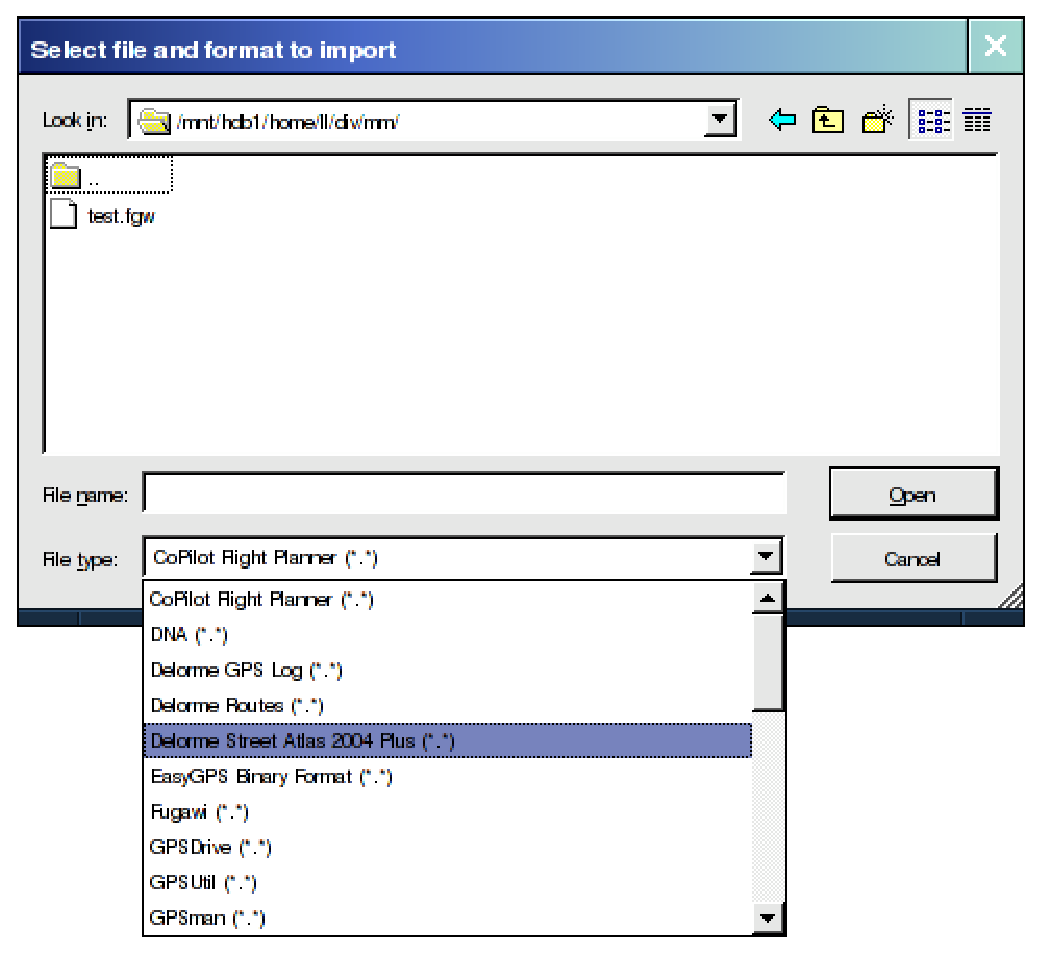
\includegraphics{qgis_user_guide_images/plugins_gps/importdialog}
\end{figure}



\subsection{Downloading GPS data from a device}

QGIS can use GPSBabel to download data from a GPS device directly
into vector layers. For this you use the tool \emph{Download from
GPS} (see Figure \ref{figure_download}), where you select your type
of GPS device, the port that it is connected to, the feature type
that you want to download, the GPX file where the data should be stored,
and the name of the new layer.

%
\begin{figure}

\caption{\label{figure_download}The download tool}

\includegraphics[%
  scale=0.5]{qgis_user_guide_images/plugins_gps/download}
\end{figure}


The device type you select in the GPS device menu determines how GPSBabel
tries to communicate with the device. If none of the device types
works with your GPS device you can create a new type (see section
\ref{sec:Defining-new-device}).

The port is a file name or some other name that your operating system
uses as a reference to the physical port in your computer that the
GPS device is connected to. On Linux this is something like /dev/ttyS0
or /dev/ttyS1 and on Windows it's COM1 or COM2.

When you click OK the data will be downloaded from the device and
appear as a layer in QGIS.


\subsection{Uploading GPS data to a device}

You can also upload data directly from a vector layer in QGIS to a
GPS device, using the tool \emph{Upload to GPS}. The layer must be
a GPX layer. To do this you simply select the layer that you want
to upload, the type of your GPS device, and the port that it's connected
to. Just as with the download tool you can specify new device types
if your device isn't in the list.

This tool is very useful together with the vector editing capabilities
of QGIS. You can load a map, create some waypoints and routes, and
then upload them and use them in your GPS device.


\subsection{\label{sec:Defining-new-device}Defining new device types}

There are lots of different types of GPS devices. The QGIS developers
can't test all of them, so if you have one that does not work with
any of the device types listed in the download and upload tools you
can define your own device type for it. You do this by using the \emph{GPS
device editor}, which you start by clicking the \emph{Edit devices}
button in the download or the upload window.

To define a new device you simply click the \emph{New device} button,
enter a name, a download command, and an upload command for your device,
and click the \emph{Update device} button. 

The name will be listed in the device menus in the upload and download
windows, and can be any string. 

The download command is the command that is used to download data
from the device to a GPX file. This will probably be a GPSBabel command,
but you can use any other command line program that can create a GPX
file. QGIS will replace the keywords \emph{\%type}, \emph{\%in}, and
\emph{\%out} when it runs the command.

\emph{\%type} will be replaced by {}``-w'' if you are downloading
waypoints, {}``-r'' if you are downloading routes, and {}``-t''
if you are downloading tracks. These are command line options that
tell GPSBabel which feature type to download. 

\emph{\%in} will be replaced by the port name that you choose in the
download window, and \emph{\%out} will be replaced by the name you
choose for the GPX file that the downloaded data should be stored
in. So if you create a device type with the download command {}``gpsbabel
\%type -i garmin -o gpx \%in \%out'' (this is actually the download
command for the predefined device type {}``Garmin serial'') and
then use it to download waypoints from port {}``/dev/ttyS0'' to
the file {}``output.gpx'', QGIS will replace the keywords and run
the command {}``gpsbabel -w -i garmin -o gpx /dev/ttyS0 output.gpx''.

The upload command is the command that is used to upload data to the
device. The same keywords are used, but \emph{\%in} is now replaced
by the name of the GPX file for the layer that is being uploaded,
and \emph{\%out} is replaced by the port name. You can learn more
about GPSBabel and it's available command line options at \url{http://www.gpsbabel.org}

Once you have created a new device type it will appear in the device
lists for the download and upload tools.
 not translated yet
%% html: Beginning of file: `index.html'
    
\section{Using the Delmited Text Plugin}
\label{f0}    

The Delimited Text plugin allows you to load a delimited text file  as a layer in QGIS. 
    
\subsection{Requirements}
To view a delimited text file as layer, the text file must contain:
\begin{enumerate}      
\item A delimited header row of field names. This must be the first line in the text file     \item The header row must contain an X and Y field. These fields can have any name.
\item The x and y coordinates must be specified as a number. The coordinate system is not important
\end{enumerate}
An example of a valid text file might look like this:
\begin{verbatim} 
name|latdec|longdec|cell|
196 mile creek|61.89806|-150.0775|tyonek d-1 ne|
197 1/2 mile creek|61.89472|-150.09972|tyonek d-1 ne|
a b mountain|59.52889|-135.28333|skagway c-1 sw|
apw dam number 2|60.53|-145.75167|cordova c-5 sw|
apw reservoir|60.53167|-145.75333|cordova c-5 sw|
apw reservoir|60.53|-145.75167|cordova c-5 sw|
aaron creek|56.37861|-131.96556|bradfield canal b-6|
aaron island|58.43778|-134.81944|juneau b-3 ne|
aats bay|55.905|-134.24639|craig d-7|
\end{verbatim}


Some items of note about the text file are:

\begin{enumerate}        
\item  The example text file uses \mbox{$|$} as delimter. Any character can be used to         delimit the fields.
\item The first row is the header row. It contains the fields name, latdec, longdec, and cell
\item No quotes ({\tt{}"{}}) are used to delimit text fields
\item The x coordinates are contained in the {\em longdec} field
\item The y coordinates are contained in the {\em latdec} field
\end{enumerate}


\subsection{Using the Plugin}
To use the plugin you must have QGIS running and use the Plugin Manager to load the plugin:

Start QGIS, then Open the Plugin Manager by choosing the {\em Tools\mbox{$|$}Plugin Manager} menu. The Plugin Manager displays a list of available plugins. Plugins that are already loaded have a checkmark to the left of their name. Click on the checkbox to the left of the {\em Add Delimited Text Layer} plugin and click Ok to load it as shown in Figure \ref{fig:plugin_manager}.

\begin{figure}[h]
   \begin{center}
   \caption{Plugin Manager Dialog}
   \label{fig:plugin_manager}
   \smallskip
   
\includegraphics[scale=0.6]{qgis_user_guide_images/plugins_delimited_text/plugin_manager}
   \end{center}  
\end{figure}


A new toolbar icon is now present:

\includegraphics[scale=0.8]{qgis_user_guide_images/plugins_delimited_text/toolbar_icon}
Click on the icon to open the Delimited Text dialog as shown in Figure \ref{fig:delim_text_plugin_dialog}.

\begin{figure}[h]
   \begin{center}
   \caption{Delimited Text Dialog}\label{fig:delim_text_plugin_dialog}\smallskip
   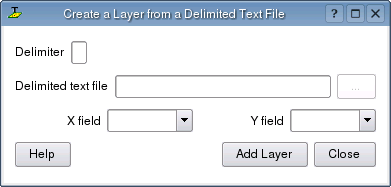
\includegraphics[scale=0.6]{qgis_user_guide_images/plugins_delimited_text/dialog}            
   \end{center}  
\end{figure}

  
First select the file to import by clicking on the ellipsis button: 
\includegraphics[scale=0.5]{qgis_user_guide_images/plugins_delimited_text/ellipsis}
Select the desired text file from the file dialog
Once the file is selected, the plugin attempts to parse the file using the last
used delimiter, in this case \mbox{$|$} (Figure
\ref{fig:delim_text_file_selected}).
\begin{figure}[h]
   \begin{center}
   \caption{File Selected}\label{fig:delim_text_file_selected}\smallskip
   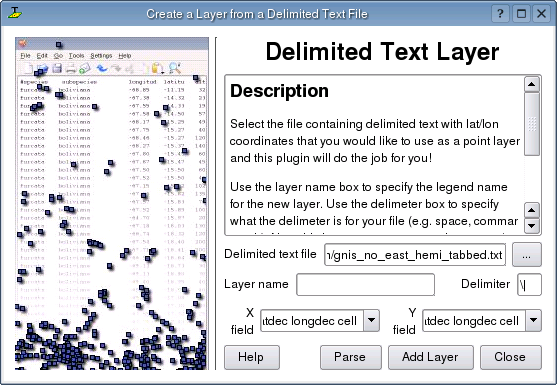
\includegraphics[scale=0.6]{qgis_user_guide_images/plugins_delimited_text/file_selected}   
   \end{center}  
\end{figure}

In this case the delimiter \mbox{$|$} is not correct for the file. The file is actually tab delimited. Note that the X and Y field drop down boxes do not contain valid field names.
To properly parse the file, change the delimiter to tab using
\mbox{$\backslash$}t (this is a regular expression for the tab character). After
changing the delimiter, click {\em Parse}.
The drop down boxes now contain the fields properly parsed as shown in Figure
\ref{fig:delim_text_file_selected2}.

Choose the X and Y fields from the drop down boxes and enter a Layer name as
shown in Figure \ref{fig:delim_text_file_selected3}. To add the layer to the
map, click {\em Add Layer}. The delimited text file now behaves as any other map
layer in QGIS (Figure \ref{fig:layer_added}).
\begin{figure}[h]
   \begin{center}
   \caption{Fields Parsed from Text File}\label{fig:delim_text_file_selected2}\smallskip
   \includegraphics[scale=0.6]{qgis_user_guide_images/plugins_delimited_text/file_selected2}
   \end{center}  
\end{figure}

\begin{figure}[h]
   \begin{center}
   \caption{Selecting the X and Y Fields}\label{fig:delim_text_file_selected3}\smallskip
   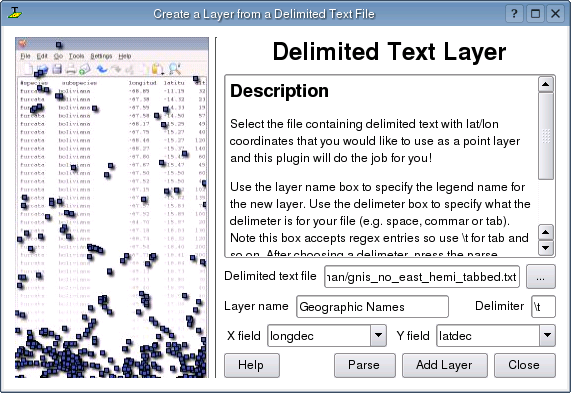
\includegraphics[scale=0.6]{qgis_user_guide_images/plugins_delimited_text/file_selected3}
   \end{center}  
\end{figure}
\begin{figure}[h]
   \begin{center}
   \caption{Delimited Text Layer Added to QGIS}\label{fig:layer_added}\smallskip
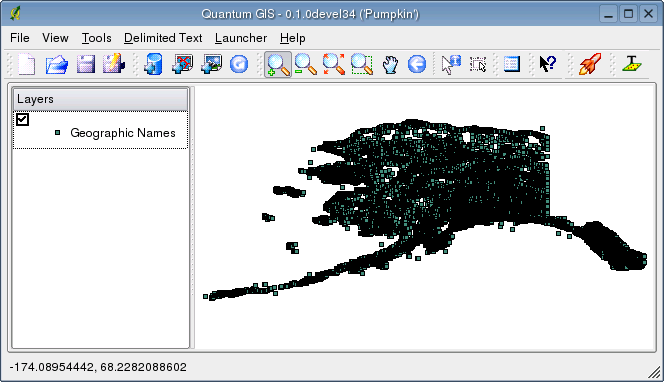
\includegraphics[scale=0.6]{qgis_user_guide_images/plugins_delimited_text/layer_added}
   \end{center}  
\end{figure}



% html: End of file: `index.html'
 not translated yet
%end of plugin docs
%\chapter{Help and Support}

QGIS is still under active development and as such it won't always work like you expect it to.
The preferred way to get help is by joining the qgis-users mailing list Your questions will reach abroader audience and answers will benefit others. You can subscribe to the qgis-users mailing list by visiting here: http://lists.sourceforge.net/lists/listinfo/qgis-user

If you are a developer facing problems of a more technical nature, you may want to join the qgis-developer mailing list here: http://lists.sourceforge.net/lists/listinfo/qgis-developer

We also maintain a presence on IRC - visit us by joining the \#qgis channel on irc.freenode.net. Please wait around for a response to your question as many folks on the channel are doing other things andit may take a while for them to notice your question.
Commercial support for QGIS is available from Micro Resources 

While the qgis-users mailing list is useful for general 'how do I do xyz in QGIS' type questions, you may wish to notify us about bugs in QGIS. You can submit bug reports using the QGIS bug tracker. When reporting a bug, either login to SourceForge or, if you don't have a SourceForge id, provide an email address where we can request additional information.
Feature requests can be submitted using the feature tracker. Please bear in mind that your bug may not always enjoy the priority you might hope for (depending on its severity). Some bugs may require may require significant developer effort to remedy and the manpower is not always available for this.

If you have found a bug and fixed it yourself you can submit it to the QGIS Sourceforge patch queue where someone will review it and apply it to QGIS. Please dont be alarmed if your patch is not applied straight away - developers may be tied up with other committments.

There is also a community site for QGIS where we encourage QGIS users to share their experiences and provide case studies about how they are using QGIS. The community site is available at: http://community.qgis.org 

Lastly, we maintain a WIKI web site at http://wiki.qgis.org where you can find a variety of useful information relating to QGIS development, release plans, links to download sites and so on. not translated yet

\appendix



%\chapter{Supported Data Formats}\label{appdx_data_formats}
\section{Supported OGR Formats}\label{appdx_ogr} \index{ogr!supported formats}
At the date of this document, the following formats are supported by the OGR
library. Formats known to work in QGIS are indicated in \textbf{bold}.

\begin{compactitem}
\item \textbf{Arc/Info Binary Coverage}
\item Comma Separated Value (.csv) 
\item DODS/OPeNDAP
\item \textbf{ESRI Shapefile}
\item FMEObjects Gateway
\item GML
\item IHO S-57 (ENC)
\item \textbf{Mapinfo File}
\item Microstation DGN
\item OGDI Vectors
\item ODBC
\item Oracle Spatial
\item PostgreSQL\footnote{QGIS implements its own PostgreSQL functions. OGR should be built without PostgreSQL support}
\item \textbf{SDTS}
\item SQLite
\item UK .NTF
\item U.S. Census TIGER/Line
\item VRT - Virtual Datasource
\end{compactitem}
\section{GDAL Raster Formats}\label{appdx_gdal}\index{rasters!supported formats}
At the date of this document, the following formats are supported by the GDAL
library. Note that not all of these format may work in QGIS for various reasons.
For example, some require external commercial libraries. Only those formats that
have been well tested will appear in the list of file types when loading a
raster into QGIS. Other untested formats can be loaded by selecting the
\textsl{All other files (*)} filter. Formats known to work in QGIS are indicated
in \textbf{bold}.

\begin{compactitem}
\item \textbf{Arc/Info ASCII Grid}
\item \textbf{Arc/Info Binary Grid (.adf)}
\item Microsoft Windows Device Independent Bitmap (.bmp)
\item BSB Nautical Chart Format (.kap)
\item VTP Binary Terrain Format (.bt)
\item CEOS (Spot for instance)
\item First Generation USGS DOQ (.doq)
\item New Labelled USGS DOQ (.doq)
\item Military Elevation Data (.dt0, .dt1)
\item ERMapper Compressed Wavelets (.ecw)
\item ESRI .hdr Labelled
\item ENVI .hdr Labelled Raster
\item Envisat Image Product (.n1)
\item EOSAT FAST Format
\item FITS (.fits)
\item Graphics Interchange Format (.gif)
\item \textbf{GRASS Rasters}\footnote{GRASS raster support is supplied by the QGIS GRASS data provider plugin} 
\item \textbf{TIFF / GeoTIFF (.tif)}
\item Hierarchical Data Format Release 4 (HDF4)
\item \textbf{Erdas Imagine (.img)}
\item Atlantis MFF2e
\item Japanese DEM (.mem)
\item \textbf{JPEG JFIF (.jpg)}
\item JPEG2000 (.jp2, .j2k)
\item JPEG2000 (.jp2, .j2k)
\item NOAA Polar Orbiter Level 1b Data Set (AVHRR)
\item Erdas 7.x .LAN and .GIS
\item In Memory Raster
\item Atlantis MFF
\item Multi-resolution Seamless Image Database  MrSID
\item NITF
\item NetCDF
\item OGDI Bridge
\item PCI .aux Labelled
\item PCI Geomatics Database File
\item Portable Network Graphics (.png)
\item Netpbm (.ppm,.pgm)
\item \textbf{USGS SDTS DEM (*CATD.DDF)}
\item SAR CEOS
\item \textbf{USGS ASCII DEM (.dem)}
\item X11 Pixmap (.xpm)

\end{compactitem}
\clearpage not translated yet
%\chapter{Gnu Public License}
\label{gpl_appendix}
\index{license!GPL}
\begin{small}
\begin{center}
GNU GENERAL PUBLIC LICENSE

Version 2, June 1991


Copyright (C) 1989, 1991 Free Software Foundation, Inc.  
59 Temple Place - Suite 330, Boston, MA  02111-1307, USA


Everyone is permitted to copy and distribute verbatim copies
of this license document, but changing it is not allowed.
\end{center}
Preamble

The licenses for most software are designed to take away your freedom to share and change it. By contrast, the GNU General Public License is intended to guarantee your freedom to share and change free software--to make sure the software is free for all its users. This General Public License applies to most of the Free Software Foundation's software and to any other program whose authors commit to using it. (Some other Free Software Foundation software is covered by the GNU Library General Public License instead.) You can apply it to your programs, too.

When we speak of free software, we are referring to freedom, not price. Our General Public Licenses are designed to make sure that you have the freedom to distribute copies of free software (and charge for this service if you wish), that you receive source code or can get it if you want it, that you can change the software or use pieces of it in new free programs; and that you know you can do these things.

To protect your rights, we need to make restrictions that forbid anyone to deny you these rights or to ask you to surrender the rights. These restrictions translate to certain responsibilities for you if you distribute copies of the software, or if you modify it.

For example, if you distribute copies of such a program, whether gratis or for a fee, you must give the recipients all the rights that you have. You must make sure that they, too, receive or can get the source code. And you must show them these terms so they know their rights.

We protect your rights with two steps: (1) copyright the software, and (2) offer you this license which gives you legal permission to copy, distribute and/or modify the software.

Also, for each author's protection and ours, we want to make certain that everyone understands that there is no warranty for this free software. If the software is modified by someone else and passed on, we want its recipients to know that what they have is not the original, so that any problems introduced by others will not reflect on the original authors' reputations.

Finally, any free program is threatened constantly by software patents. We wish to avoid the danger that redistributors of a free program will individually obtain patent licenses, in effect making the program proprietary. To prevent this, we have made it clear that any patent must be licensed for everyone's free use or not licensed at all.

The precise terms and conditions for copying, distribution and modification follow.
TERMS AND CONDITIONS FOR COPYING, DISTRIBUTION AND MODIFICATION

0. This License applies to any program or other work which contains a notice placed by the copyright holder saying it may be distributed under the terms of this General Public License. The "Program", below, refers to any such program or work, and a "work based on the Program" means either the Program or any derivative work under copyright law: that is to say, a work containing the Program or a portion of it, either verbatim or with modifications and/or translated into another language. (Hereinafter, translation is included without limitation in the term "modification".) Each licensee is addressed as "you".

Activities other than copying, distribution and modification are not covered by this License; they are outside its scope. The act of running the Program is not restricted, and the output from the Program is covered only if its contents constitute a work based on the Program (independent of having been made by running the Program). Whether that is true depends on what the Program does.

1. You may copy and distribute verbatim copies of the Program's source code as you receive it, in any medium, provided that you conspicuously and appropriately publish on each copy an appropriate copyright notice and disclaimer of warranty; keep intact all the notices that refer to this License and to the absence of any warranty; and give any other recipients of the Program a copy of this License along with the Program.

You may charge a fee for the physical act of transferring a copy, and you may at your option offer warranty protection in exchange for a fee.

2. You may modify your copy or copies of the Program or any portion of it, thus forming a work based on the Program, and copy and distribute such modifications or work under the terms of Section 1 above, provided that you also meet all of these conditions:

    a) You must cause the modified files to carry prominent notices stating that you changed the files and the date of any change. 

    b) You must cause any work that you distribute or publish, that in whole or in part contains or is derived from the Program or any part thereof, to be licensed as a whole at no charge to all third parties under the terms of this License. 

    c) If the modified program normally reads commands interactively when run, you must cause it, when started running for such interactive use in the most ordinary way, to print or display an announcement including an appropriate copyright notice and a notice that there is no warranty (or else, saying that you provide a warranty) and that users may redistribute the program under these conditions, and telling the user how to view a copy of this License. (Exception: if the Program itself is interactive but does not normally print such an announcement, your work based on the Program is not required to print an announcement.) 

These requirements apply to the modified work as a whole. If identifiable sections of that work are not derived from the Program, and can be reasonably considered independent and separate works in themselves, then this License, and its terms, do not apply to those sections when you distribute them as separate works. But when you distribute the same sections as part of a whole which is a work based on the Program, the distribution of the whole must be on the terms of this License, whose permissions for other licensees extend to the entire whole, and thus to each and every part regardless of who wrote it.

Thus, it is not the intent of this section to claim rights or contest your rights to work written entirely by you; rather, the intent is to exercise the right to control the distribution of derivative or collective works based on the Program.

In addition, mere aggregation of another work not based on the Program with the Program (or with a work based on the Program) on a volume of a storage or distribution medium does not bring the other work under the scope of this License.

3. You may copy and distribute the Program (or a work based on it, under Section 2) in object code or executable form under the terms of Sections 1 and 2 above provided that you also do one of the following:

    a) Accompany it with the complete corresponding machine-readable source code, which must be distributed under the terms of Sections 1 and 2 above on a medium customarily used for software interchange; or, 

    b) Accompany it with a written offer, valid for at least three years, to give any third party, for a charge no more than your cost of physically performing source distribution, a complete machine-readable copy of the corresponding source code, to be distributed under the terms of Sections 1 and 2 above on a medium customarily used for software interchange; or, 

    c) Accompany it with the information you received as to the offer to distribute corresponding source code. (This alternative is allowed only for noncommercial distribution and only if you received the program in object code or executable form with such an offer, in accord with Subsection b above.) 

The source code for a work means the preferred form of the work for making modifications to it. For an executable work, complete source code means all the source code for all modules it contains, plus any associated interface definition files, plus the scripts used to control compilation and installation of the executable. However, as a special exception, the source code distributed need not include anything that is normally distributed (in either source or binary form) with the major components (compiler, kernel, and so on) of the operating system on which the executable runs, unless that component itself accompanies the executable.

If distribution of executable or object code is made by offering access to copy from a designated place, then offering equivalent access to copy the source code from the same place counts as distribution of the source code, even though third parties are not compelled to copy the source along with the object code.

4. You may not copy, modify, sublicense, or distribute the Program except as expressly provided under this License. Any attempt otherwise to copy, modify, sublicense or distribute the Program is void, and will automatically terminate your rights under this License. However, parties who have received copies, or rights, from you under this License will not have their licenses terminated so long as such parties remain in full compliance.

5. You are not required to accept this License, since you have not signed it. However, nothing else grants you permission to modify or distribute the Program or its derivative works. These actions are prohibited by law if you do not accept this License. Therefore, by modifying or distributing the Program (or any work based on the Program), you indicate your acceptance of this License to do so, and all its terms and conditions for copying, distributing or modifying the Program or works based on it.

6. Each time you redistribute the Program (or any work based on the Program), the recipient automatically receives a license from the original licensor to copy, distribute or modify the Program subject to these terms and conditions. You may not impose any further restrictions on the recipients' exercise of the rights granted herein. You are not responsible for enforcing compliance by third parties to this License.

7. If, as a consequence of a court judgment or allegation of patent infringement or for any other reason (not limited to patent issues), conditions are imposed on you (whether by court order, agreement or otherwise) that contradict the conditions of this License, they do not excuse you from the conditions of this License. If you cannot distribute so as to satisfy simultaneously your obligations under this License and any other pertinent obligations, then as a consequence you may not distribute the Program at all. For example, if a patent license would not permit royalty-free redistribution of the Program by all those who receive copies directly or indirectly through you, then the only way you could satisfy both it and this License would be to refrain entirely from distribution of the Program.

If any portion of this section is held invalid or unenforceable under any particular circumstance, the balance of the section is intended to apply and the section as a whole is intended to apply in other circumstances.

It is not the purpose of this section to induce you to infringe any patents or other property right claims or to contest validity of any such claims; this section has the sole purpose of protecting the integrity of the free software distribution system, which is implemented by public license practices. Many people have made generous contributions to the wide range of software distributed through that system in reliance on consistent application of that system; it is up to the author/donor to decide if he or she is willing to distribute software through any other system and a licensee cannot impose that choice.

This section is intended to make thoroughly clear what is believed to be a consequence of the rest of this License.

8. If the distribution and/or use of the Program is restricted in certain countries either by patents or by copyrighted interfaces, the original copyright holder who places the Program under this License may add an explicit geographical distribution limitation excluding those countries, so that distribution is permitted only in or among countries not thus excluded. In such case, this License incorporates the limitation as if written in the body of this License.

9. The Free Software Foundation may publish revised and/or new versions of the General Public License from time to time. Such new versions will be similar in spirit to the present version, but may differ in detail to address new problems or concerns.

Each version is given a distinguishing version number. If the Program specifies a version number of this License which applies to it and "any later version", you have the option of following the terms and conditions either of that version or of any later version published by the Free Software Foundation. If the Program does not specify a version number of this License, you may choose any version ever published by the Free Software Foundation.

10. If you wish to incorporate parts of the Program into other free programs whose distribution conditions are different, write to the author to ask for permission. For software which is copyrighted by the Free Software Foundation, write to the Free Software Foundation; we sometimes make exceptions for this. Our decision will be guided by the two goals of preserving the free status of all derivatives of our free software and of promoting the sharing and reuse of software generally.

NO WARRANTY

11. BECAUSE THE PROGRAM IS LICENSED FREE OF CHARGE, THERE IS NO WARRANTY FOR THE PROGRAM, TO THE EXTENT PERMITTED BY APPLICABLE LAW. EXCEPT WHEN OTHERWISE STATED IN WRITING THE COPYRIGHT HOLDERS AND/OR OTHER PARTIES PROVIDE THE PROGRAM "AS IS" WITHOUT WARRANTY OF ANY KIND, EITHER EXPRESSED OR IMPLIED, INCLUDING, BUT NOT LIMITED TO, THE IMPLIED WARRANTIES OF MERCHANTABILITY AND FITNESS FOR A PARTICULAR PURPOSE. THE ENTIRE RISK AS TO THE QUALITY AND PERFORMANCE OF THE PROGRAM IS WITH YOU. SHOULD THE PROGRAM PROVE DEFECTIVE, YOU ASSUME THE COST OF ALL NECESSARY SERVICING, REPAIR OR CORRECTION.

12. IN NO EVENT UNLESS REQUIRED BY APPLICABLE LAW OR AGREED TO IN WRITING WILL ANY COPYRIGHT HOLDER, OR ANY OTHER PARTY WHO MAY MODIFY AND/OR REDISTRIBUTE THE PROGRAM AS PERMITTED ABOVE, BE LIABLE TO YOU FOR DAMAGES, INCLUDING ANY GENERAL, SPECIAL, INCIDENTAL OR CONSEQUENTIAL DAMAGES ARISING OUT OF THE USE OR INABILITY TO USE THE PROGRAM (INCLUDING BUT NOT LIMITED TO LOSS OF DATA OR DATA BEING RENDERED INACCURATE OR LOSSES SUSTAINED BY YOU OR THIRD PARTIES OR A FAILURE OF THE PROGRAM TO OPERATE WITH ANY OTHER PROGRAMS), EVEN IF SUCH HOLDER OR OTHER PARTY HAS BEEN ADVISED OF THE POSSIBILITY OF SUCH DAMAGES. 
\end{small}
 not included yet
%\section{Quantum GIS Qt exception for GPL}
\index{license!exception}
\label{qgis_qt_exception_appendix}

\begin{quotation}
In addition, as a special exception, the QGIS Development Team gives
permission to link the code of this program with the Qt library,
including but not limited to the following versions (both free and
commercial): Qt/Non-commerical Windows, Qt/Windows, Qt/X11, Qt/Mac, and
Qt/Embedded (or with modified versions of Qt that use the same license
as Qt), and distribute linked combinations including the two. You must
obey the GNU General Public License in all respects for all of the code
used other than Qt. If you modify this file, you may extend this
exception to your version of the file, but you are not obligated to do
so. If you do not wish to do so, delete this exception statement from
your version.
\end{quotation} 
 not translated yet
%install guide is a special case because we are snarfing it
%out of a separate document, we need to add the chapter here
\chapter{In�tala�n� pr�ru�ka QGIS}
\label{install_guide}
%% vim:textwidth=76:autoindent
\section{Introduction}\label{label_introduction}
The majority of this document is devoted to describing how to build QGIS 0.7
(\textit{`Seamus'}) from the source distribution. These instructions are for
Linux/Unix and other POSIX systems which have the required build
environment. If you are building on FreeBSD, see
\url{http://community.qgis.org/buildingOnFreeBSD.html} for hints and further
information.

Installing on Windows and Mac OS X is a simple process as described
below.

You don't have to build all the QGIS dependencies from source. If your
platform provides packages at an acceptable version for the needed
dependencies, you can install them prior to building QGIS. Make sure you
also install the "development" package (if separate from the main package)
for each dependency. QGIS needs the header files from these packages in
order to build. 

The latest version of this document can always be found at
\url{http://qgis.org/docs/install.html}.
%\textsc{NOTE - All of the required packages for SuSE 9.1 are available at
%}\url{ftp://ftp.lingis.org}
\subsection{Installing Windows Version}
Installing the Windows version of QGIS is simply a matter of running the
user friendly setup wizard. See the README.WIN32 file for additional
information regarding the Windows version of QGIS. At version 0.7, the GRASS
plugin is not available in Windows. Work on including the plugin in the next
version of QGIS is under way.


\subsection{Installing Mac OS X Version}
To install the compressed disk image containing the OSX version of QGIS,
double-click to expand and mount the image, then drag QGIS application to
your hard drive. If you want to build from source on Mac OS X, see
\url{http://wiki.qgis.org/qgiswiki/BuildingOnMacOsX}. Installing the
compressed disk image is the easiest method and gives you the full
functionality of QGIS and all plugins, including GRASS. See the README file
included on the disk image for additional instructions.

%This document does not contain instructions for building the GRASS plugins. Information on building the GRASS plugin with raster and vector support can be found in the \textit{Building QGIS with GRASS Support} document, available at \url{http://community.qgis.org/grass_plugin}. 

\subsection{Building from Source}
The remainder of this document deals with compiling and installing QGIS from the
source code. Specifically this applies to Linux/Unix systems.

At 0.7, there are two new requirements: SQLite and Proj4. These must be built and installed prior to configuring QGIS.

QGIS can be installed with three levels of support for data stores:
\begin{enumerate}
\item Basic raster and vector support (GDAL and OGR formats)
\item PostreSQL/GEOS/PostGIS 
\item GRASS raster and vector support
\end{enumerate} 

Basic support uses the GDAL/OGR libraries and supports many raster and
vector formats. For more information on the available formats, see
\url{http://gdal.maptools.org/formats_list.html} and
\url{http://gdal.maptools.org/ogr/ogr_formats.html}.

PostgreSQL/PostGIS support allows you to store spatial data in a PostgreSQL database. GRASS support provides access to GRASS mapsets. 

\textbf{Note:} - If you plan to build QGIS with GRASS support, version 1.2.6 or higher of GDAL must be used. 
  
Each of the requirements is discussed below. Note that the information given below is abstracted from the installation documentation for each of the libraries. See the install information for each library to get detailed instructions. In the documentation below, the file names and versions used are examples.


If you are building QGIS without PostgreSQL or GRASS support, skip to the section on Installing GDAL/OGR. 
\section{Getting QGIS}
QGIS is available in both source and package format from \url{http://qgis.org}. 

In addition, packages for many Linux distributions are independently maintained in various locations. See 
the \textit{Download} section on \url{http://qgis.org} for the latest information on package locations.

Packages for most of the software/libraries discussed below can be found for almost all Linux distributions. While it is possible to mix compiling from source and installing packages to meet the requirements for QGIS, sometimes this becomes tricky. Following the steps below will generally ensure a successful installation. If you are using SuSE 9.1, the LinGIS distribution \url{ftp://ftp.lingis.org} is a good choice for installing QGIS and its dependencies.

For information on installing dependencies and building QGIS on FreeBSD, see
\textit{Building QGIS on FreeBSD} on \url{http://community.qgis.org}.

  \section{PostgreSQL}
  QGIS uses the latest features of PostgreSQL. For this reason, version 8.0.x or higher is recommended with QGIS version 0.7. If you choose to add PostgreSQL, you must also install PostGIS (see below). 
  \begin{enumerate}
  \item Download PostgreSQL source from www.postgresql.org 
  \item Extract the source 
  \begin{verbatim}
  tar -xzf postgresql-8.0.1.tar.gz
  \end{verbatim}

  \item Change to the source directory 
  \begin{verbatim}
  cd postgresql-8.0.1
  \end{verbatim}

  \item Configure PostgreSQL:
  \begin{verbatim}
  ./configure --prefix=/usr/local/pgsql 
  \end{verbatim}

  \item Build
  \begin{verbatim}
  make
  \end{verbatim}

  \item Install
  \begin{verbatim}
  make install
  \end{verbatim}

\item As root, create the postgres user and setup the database (following taken from PostgreSQL INSTALL file with modification)
  \begin{itemize} 
  \item Create the postgres user 
  \begin{verbatim}
  adduser postgres
  \end{verbatim}

  \item Create the directory for the PostgreSQL database 
  \begin{verbatim}
  mkdir /usr/local/pgsql/data
  \end{verbatim}

  \item Change ownership of the data directory to the postgres user
  \begin{verbatim}
  chown postgres /usr/local/pgsql/data
  \end{verbatim}

\item su to the postgres user (or login as postgres)
  \begin{verbatim}
  su - postgres
  \end{verbatim}

  \item Change to the PostgreSQL install directory 
  \begin{verbatim}
  cd /usr/local/pgsql
  \end{verbatim}

  \item Initialize the database 
  \begin{verbatim}
  ./bin/initdb -D /usr/local/pgsql/data
  \end{verbatim}

  \item Start the PostgreSQL daemon 
  \small
  \begin{verbatim}
  ./bin/pg_ctl start  -o "-i" -D /usr/local/pgsql/data -l /home/postgres/serverlog 
  \end{verbatim} 
  
  \item Create the test database
  
  \begin{verbatim}
  ./bin/createdb test
  \end{verbatim}
  \normalsize
  \end{itemize}
  \item PostgreSQL should now be running. Logon as the postgres user (or use su - postgres). You should be able to connect to the test database and execute a test query with the following commands: 

  \begin{verbatim}
  psql test
  select version();
  version
  -------------------------------------------------------------------------------------
  PostgreSQL 8.0.1 on i686-pc-linux-gnu, compiled by GCC gcc (GCC) 3.3.1 (SuSE Linux)
(1 row)

  \q
  \end{verbatim}


  \item PostgreSQL install is done
  \end{enumerate}

  \section{GEOS}

  \textbf{Note:} As of version 0.6, GEOS is a requirement in order to build QGIS.
  
  QGIS uses GEOS to properly fetch features from the the underlying datastore
  when doing an identify or select operation.

  To install GEOS:
  \begin{enumerate}
  \item Download GEOS source from \url{http://geos.refractions.net}
  \item Untar GEOS
  \begin{verbatim}
  tar -xzf geos-2.0.0.tar.gz
  \end{verbatim}
  \item Change to the GEOS source dir
  \begin{verbatim}
  cd geos-2.0-.0
  \end{verbatim}
  \item Follow the instructions in the GEOS README file to complete the installation. Typically the install goes like this:
  \begin{verbatim}
  ./configure
  make
  make install
  \end{verbatim}

  \end{enumerate}

  \section{PostGIS}

  NOTE - You must edit the PostGIS Makefile and make sure that USE\_GEOS=1 is
  set. Also adjust GEOS\_DIR to point to your GEOS installation directory.
  \begin{enumerate}
  \item Download PostGIS source from \url{http://postgis.refractions.net} 

  \item Untar PostGIS into the contrib subdirectory of the PostgreSQL build directory. The contrib subdirectory is located in the directory created in step 3 of the PostgreSQL installation process.
  \item Change to the postgis subdirectory
  \item Edit the Makefile to enable GEOS support (see the note above)
\item PostGIS provides a manual in the doc/html subdirectory that explains the build process (see the Installation section)
  \item The quick and dirty steps to install PostGIS are:
  \begin{verbatim}
   cd contrib
   gunzip postgis-1.0.2.tar.gz 
   tar xvf postgis-1.0.2.tar 
   cd postgis-1.0.2 
   make 
   make install 
   createlang plpgsql yourtestdatabase 
   psql -d yourtestdatabase -f lwpostgis.sql 
   psql -d yourtestdatabase -f spatial_ref_sys.sql 
  \end{verbatim}
  \end{enumerate}
The \textbf{better way} to install PostGIS is to carefully follow the instructions in the PostGIS manual in the doc/html subdirectory or the online manual at \url{http://postgis.refractions.net/docs}

\section{GRASS}
If you want QGIS to support GRASS vector and raster layers, you must build GRASS prior to proceeding. 
Follow the directions on the GRASS website carefully to build version 6.0.x. Additional information and the build instructions can be found at \url{http://grass.itc.it}.
 
The GRASS software is available for download at \url{http://grass.itc.it/download.html}.
\section{Proj4}
Proj4 provides the functions needed for on the fly projection of map layers in version 0.7. To build and install Proj4, download the latest version from \url{http://proj.maptools.org}, untar the distribution and:
\begin{verbatim}
  ./configure
  make
  make install
\end{verbatim}
\section{SQLite}
Sqlite is used to manage the projections database and store persistent data such as spatial bookmarks. Download the latest (3.x) version of SQLite from \url{http://www.sqlite.org/}. Untar the distribution and:
\begin{verbatim}
  ./configure
  make
  make install
\end{verbatim}
Note - SQLite 3.x is included on Mac OS X 10.4.
\section{GDAL/OGR}
  The GDAL and OGR libraries provide support for raster and vector data formats. QGIS makes use of both of these libraries (which come bundled in one distribution).

  Note: A Linux binary of GDAL is available at \url{http://www.remotesensing.org/gdal}. If you choose to install the binary you will also need to download and unpack the source tree since QGIS needs the header files in order to compile.
  
  To install GDAL/OGR from source:
  \begin{enumerate}
  \item Download the GDAL distribution from
  \url{http://www.remotesensing.org/gdal}. You should use the latest
  version of GDAL if possible. The minimum recommended version for use
  with QGIS is 1.2.6. 

  \item Untar the distribution 
  \begin{verbatim}
    tar xfvz /../path/../gdal-x.x.x.tar.gz
  \end{verbatim}

  \item Change to the gdal-x.x.x subdirectory that was created by step 2
  \begin{verbatim}
    cd gdal-x.x.x
  \end{verbatim}

  \item Configure GDAL
  \begin{verbatim}
    ./configure 
  \end{verbatim}
  or if you want GRASS support
  \begin{verbatim}
    ./configure --with-grass=<full path to grass install>
  \end{verbatim}
  Depending on the GDAL version you are building, it may be necessary to
  specify --without-ogdi when running configure if you don't have the OGDI
  library available on your system.

  \item Build and install GDAL:
  \begin{verbatim}
    make
    su
    make install
  \end{verbatim}

  \item In order to run GDAL after installing it is necessary for the shared
  library to be findable. This can often be accomplished by setting
  LD\_LIBRARY\_PATH to include /usr/local/lib. On Linux, you can add
  /usr/local/lib (or whatever path you used for installing GDAL) to
  /etc/ld.so.conf and run ldconfig as root.

  \item Make sure that gdal-config (found in the bin subdirectory where GDAL was installed) is included in the PATH. If necessary, add the path to gdal-config to the PATH environment variable.
  \begin{verbatim}
    export PATH=/../path/../gdal-config:$PATH
  \end{verbatim}

  \item Check the install by running:
  \begin{verbatim}
    gdal-config --prefix
  \end{verbatim}

  \end{enumerate}

  If you've had problems during the installation, refer to this manual, where the whole process is described with some more detail: \url{http://www.remotesensing.org/gdal/gdal\_building.html} 

  \section{Qt}
  Qt 3.2.1 or higher is required in order to compile QGIS. You may already have Qt on your system. If so, check to see if you have version 3.2.1 or later. You can check the Qt version using the find command:
  \begin{verbatim}
  find ./ -name qglobal.h 2>/dev/null | xargs grep QT_VERSION_STR
  \end{verbatim}
  If you have the locate utility installed you can do the same more quickly using:
  \begin{verbatim}
  locate qglobal.h | xargs grep QT_VERSION_STR
  \end{verbatim}
  In either case the result should look something like this:
  \begin{verbatim}
   #define QT_VERSION_STR   "3.3.1"
   \end{verbatim} 
   In the example above, Qt 3.3.1 is installed.
   
  If Qt is not installed, you will have to install the Qt development package for your distribution. If you are not able to install the required Qt packages, you will have to build from source.
 
  To install Qt from source:
  \begin{enumerate}
  \item Download Qt from \url{http://www.trolltech.com/developer} (choose the Qt/X11 Free Edition)
  \item Unpack the distribution
  \item Follow directions provided in the distribution directory (doc/html/install-x11.html)
  \item Use whatever configure options you like but make sure you include -thread for use with QGIS. You can configure Qt with minimal options:
  \begin{verbatim}
    ./configure -thread
  \end{verbatim}

  \item Complete the installation per the instructions provided in the Qt documentation (see step 3)
  \end{enumerate}
NOTE - QGIS will not compile under Qt 4.0.x. The best choice for compiling
QGIS is Qt 3.3.x.

 \section{Building QGIS}
  
  After you have installed the required libraries, you are ready to build QGIS. Download and untar the QGIS distribution and change to the QGIS source directory. You have two options for building and installing QGIS: \textbf{Quick and Dirty} and the \textbf{right way}.
  \subsection{Quick and Dirty}
  If you don't need PostgreSQL support and have installed GDAL ,
  you can configure and build QGIS by changing to the distribution directory
  and typing:
  \begin{verbatim}./configure
    make
    make install
  \end{verbatim}
  The above assumes that the gdal-config program is in your PATH
  See the next section for the full configuration instructions.
  \subsection{Configuring QGIS the Right Way}
  To see the configure options available, change the the QGIS 
  directory and enter:
  \begin{verbatim}
    ./configure --help
   \end{verbatim}
  Among other options, there are three that are important to
  the success of the build:
  \begin{verbatim}
    --with-qtdir=DIR              Qt installation directory default=$QTDIR
    --with-gdal=path/gdal-config  Full path to 'gdal-config' script,
                                  e.g. '--with-gdal=/usr/local/bin/gdal-config'
    --with-pg=path/pg_config      PostgreSQL (PostGIS) Support
                                 (full path to pg_config)
     --with-grass=DIR             GRASS Support (full path to GRASS binary package)

  \end{verbatim}

  \subsubsection{Qt}
  The configure script will detect Qt, unless it is installed in a
  non-standard location. Setting the QTDIR environment variable will 
  make ensure that the detection succeeds. You can also specify the
  path using the --with-qtdir option. 
  \subsubsection{GDAL}
  If the gdal-config script is in the PATH, configure will automatically
  detect and configure GDAL support. If not in the path, you can specify
  the full path to gdal-config using the --with-gdal option. For example:
  \begin{verbatim}
    /configure --with-gdal=/usr/mystuff/bin/gdal-config
  \end{verbatim}
  \subsubsection{PostgreSQL}
  If the pg\_config script is in the PATH, configure will automatically
  detect and configure PostgreSQL support. If not, you can use the
  --with-pg option to specify the full path to pg\_config. For example:
  \begin{verbatim}
    ./configure --with-pg=/usr/local/psql/bin/pg_config
  \end{verbatim}
\subsubsection{GRASS}
To build QGIS with GRASS support you must specify the full path to the installed GRASS binary package:
\begin{verbatim}
    ./configure --with-grass=/usr/local/grass-6.0.0
\end{verbatim}
This assumes that GRASS is installed in the default location. Change the path to match the location of your GRASS installation.
  \subsubsection{Example Use of Configure}
  An example of use of configure for building QGIS with all options:
  \begin{verbatim}
    ./configure --prefix=/usr/local/qgis \
    --with-gdal=/usr/local/gdal/bin/gdal-config \
    --with-pg=/usr/local/psql/bin/pg_config \
    --with-grass=/usr/local/grass-6.0.0
  \end{verbatim}
  This will configure QGIS to use GDAL, GRASS, and PostgreSQL. QGIS will be
  installed in /usr/local/qgis.

  If QTDIR is set and gdal-config and pg\_config are both
  in the PATH, there is no need to use the --with-gdal and --with-pg
  options. The configure script will properly detect and configure
  GDAL and PostgreSQL. You must still use the --with-grass option if building with GRASS support.
  \subsubsection{Compiling and Installing QGIS}
  Once properly configured simply issue the following commands:
  \begin{verbatim}
    make
    make install
  \end{verbatim}
NOTE - You must do a \textit{make install} and start QGIS from the installed location. In the case of the example above, the QGIS binary resides in the bin subdirectory of the directory specified with the prefix option (/usr/local/qgis/bin).

For information on using QGIS see the QGIS User Guide.

\section{Building Plugins}
The QGIS source distribution contains a number of "core" plugins. These are built along with QGIS using the instructions above. Additional external plugins are available from the QGIS community website at \url{http://community.qgis.org}. Instructions for building an external plugin can be found at \url{http://wiki.qgis.org/qgiswiki/StepByStepBuildInstructions}. Some external plugins may include instructions on building. If so, follow the instructions provided with the plugin rather than those provided in the wiki. 
 not translated yet


\end{onehalfspace}
%\index{PostgreSQL!layer definition| \see{query builder}}
%\index{PostgreSQL!import data| \see{SPIT}}
%\index{layers!vector| \see{vector layers}}
%\index{vector layers!symbology!renderers| \see{renderers}}
\index{vrstvy!rastrov�| \see{rastre}}
%\index{attribute actions| \see{actions}}
%\index{indexes| \see{spatial index}}
\printindex
\end{document}
